\documentclass[degree=bachelor, tocarialchapter, pifootnote]{thuthesis}
% 选项
%   degree=[bachelor|master|doctor|postdoctor], % 必选,学位类型
%   secret,                % 可选(默认:关闭),是否有密级
%   tocarialchapter,       % 可选(默认:关闭),章目录中使用黑体(这项表示同时打开下面两项)
%   tocarialchapterentry,  % 可选(默认:关闭),单独控制章标题在目录中使用黑体
%   tocarialchapterpage,   % 可选(默认:关闭),单独控制章页码在目录中使用黑体
%   pifootnote,            % 可选(默认:关闭),页脚编号采用 pifont 字体符号,建议打开

% 所有其它可能用到的包都统一放到这里了,可以根据自己的实际添加或者删除。
\usepackage{thuthesis}

\usepackage{amsmath}
\usepackage{booktabs}
\usepackage{graphicx}
\usepackage{listings}
\usepackage{xcolor}
\definecolor{codebg}{rgb}{0.949, 0.949, 0.922} 
\lstset{ 
	backgroundcolor=\color{codebg},
}
\usepackage[colorinlistoftodos]{todonotes}

% 定义所有的图片文件在 figures 子目录下
\graphicspath{{figures/}}

% 可以在这里修改配置文件中的定义。导言区可以使用中文。
\def\myname{李林翼}

\begin{document}

%%% 封面部分
\frontmatter
\thusetup{
  %******************************
  % 注意:
  %   1. 配置里面不要出现空行
  %   2. 不需要的配置信息可以删除
  %******************************
  %
  %=====
  % 秘级
  %=====
  % secretlevel={秘密},
  % secretyear={10},
  %
  %=========
  % 中文信息
  %=========
  ctitle={Web API场景建模及
\\测试自动生成的研究与实现},
  cdegree={工学学士},
  cdepartment={计算机科学与技术系},
  cmajor={计算机科学与技术},
  cauthor={李林翼},
  csupervisor={白晓颖副教授},
  % cassosupervisor={陈文光教授}, % 副指导老师
  % ccosupervisor={某某某教授}, % 联合指导老师
  % 日期自动使用当前时间,若需指定按如下方式修改:
  cdate={2018年6月16日},
  %
  % 博士后专有部分
  % cfirstdiscipline={计算机科学与技术},
  % cseconddiscipline={系统结构},
  % postdoctordate={2009年7月——2011年7月},
  % id={编号}, % 可以留空: id={},
  % udc={UDC}, % 可以留空
  % catalognumber={分类号}, % 可以留空
  %
  %=========
  % 英文信息
  %=========
  etitle={Research and Implementation of Web API Scenario Modeling and Automated Test Generation},
  % 这块比较复杂,需要分情况讨论:
  % 1. 学术型硕士
  %    edegree:必须为Master of Arts或Master of Science(注意大小写)
  %             “哲学、文学、历史学、法学、教育学、艺术学门类,公共管理学科
  %              填写Master of Arts,其它填写Master of Science”
  %    emajor:“获得一级学科授权的学科填写一级学科名称,其它填写二级学科名称”
  % 2. 专业型硕士
  %    edegree:“填写专业学位英文名称全称”
  %    emajor:“工程硕士填写工程领域,其它专业学位不填写此项”
  % 3. 学术型博士
  %    edegree:Doctor of Philosophy(注意大小写)
  %    emajor:“获得一级学科授权的学科填写一级学科名称,其它填写二级学科名称”
  % 4. 专业型博士
  %    edegree:“填写专业学位英文名称全称”
  %    emajor:不填写此项
  edegree={Bachelor of Engineering},
  emajor={Computer Science and Technology},
  eauthor={Linyi Li},
  esupervisor={Associate Professor Xiaoying Bai},
  % eassosupervisor={Chen Wenguang},
  % 日期自动生成,若需指定按如下方式修改:
  % edate={December, 2005}
  %
  % 关键词用“英文逗号”分割
  ckeywords={Web API, 场景建模, 自动化测试, 软件测试, OpenAPI},
  ekeywords={Web API, Scenario Modeling, Automated Testing, Software Testing, OpenAPI}
}

% 定义中英文摘要和关键字
\begin{cabstract}
Web API在互联网软件中正被广泛应用. Web API可作为公开服务提供, 并集成于应用中, 满足各种用户需求. 因此, 作为应用的基础构件, web API的测试十分必要. 然而, 由于web API调用方式多样, 且常常动态更新与修改, 故其测试需要使用大量测试用例, 并需要定期回归测试, 因此, 手动测试具有很高代价.

本文提出了一种基于场景模型的web API自动化测试方法: 首先, 基于概率有限状态自动机进行扩展, 对API的使用进行了场景建模, 本文形式化定义的场景模型可以有效描述API数据流与控制流的约束、断言和状态转移, 并反映API的使用模式与频率. 然后提出了基于场景模型自动化生成测试用例的方法, 其包括请求数据与调用序列的自动化生成两方面. 最后, 本文介绍了Lapis工具, 它提供了该方法的完整实现. 利用该工具, 本文在实际web API服务上对模型和方法进行了评估, 从多个方面验证了其有效性和使用价值. 最后, 本文总结并展望了基于此场景模型进一步提高测试自动化程度和测试生成质量的研究方向.

  
\end{cabstract}

% 如果习惯关键字跟在摘要文字后面,可以用直接命令来设置,如下:
% \ckeywords{\TeX, \LaTeX, CJK, 模板, 论文}

\begin{eabstract}
Web API has been widely used for Internet software. Once published as open services, web APIs can be integrated into various applications to accommodate diversified usage scenarios. Therefore, as fundamental components, web API testing is inevitable. However, due to diversity of web API calling convention and high frequency of updates and modifications, web API testing requires a large number of test cases and frequent regression testing. Therefore, manual testing is expensive.

This thesis proposed a scenario-based approach for web API testing. Firstly, it extended probabilistic finite-state automata to model API usage. The formally defined scenario model facilitates the expression of API control flow and data flow constraints as well as assertions and state transitions. Meanwhile, the model could reveal the API usage pattern and usage frequency. Secondly, it proposed an approach to generate test cases from scenario model automatically, which includes request data automated generation and calling sequence automated generation. Lastly, it introduced the tool Lapis, which provides a full implementation of the approach. With the tool, we evaluated scenario model and approach on real web API services. The performance revealed the validity and valuable of them in several aspects. The thesis concluded with a brief summary and a discussion on how to further improve testing automaticity and quality based on proposed scenario model.
\end{eabstract}

% \ekeywords{\TeX, \LaTeX, CJK, template, thesis}

% 如果使用授权说明扫描页,将可选参数中指定为扫描得到的 PDF 文件名,例如:
% \makecover[scan-auth.pdf]
\makecover[scan-auth.pdf]

%% 目录
\tableofcontents

%% 符号对照表
\begin{denotation}[3cm]
\item[API] 应用程序编程接口
\item[SUT] 被测系统 
\item[JVM] Java虚拟机 
\item[JVM Languages] Java虚拟机语言, 指可被编译为Java字节码的语言, 如Java, Scala, Kotlin等 

\item[Heuristics] 启发值, 多用于启发式算法与搜索算法 
\item[Fitness Value] 适应度值 
\item[Test Case] 测试用例 
\item[Test Oracle] 测试参照, 即测试中用于参照的目标 
\item[Text Archive] 测试档案, 一般是一些测试用例的集合 
\item[Resource] 资源 
\item[Coverage] 覆盖率 
\item[Bug] 故障 
\item[Empirical Study] 实证研究 
\item[Endpoint] 端点, 本文中指API服务端点, 通常为一个具体的API
\item[Mock] 模拟 
\item[Statement Coverage] 语句/代码覆盖率 
\item[Code Instrumentation] 代码测量 
\item[Evolutionary Algorithm] 进化算法 
\end{denotation}



%%% 正文部分
\mainmatter

\chapter{引言}

	\section{背景介绍}
    
        近年来, 云计算和移动计算获得了空前的发展, 面向服务的体系结构(SOA)已经成为了云计算和移动计算的主流架构\cite{wintergreen17}. 预计至2020年, SOA市场的规模将达到164亿美元. 而云计算业务的市场规模将于2021年达到715.5亿美元\cite{skyhighnetworks18azure}. 面向服务的体系结构经常使用web API的形式对外提供开放服务\cite{hamza15}, 这些web API常常使用SOAP(简单对象访问协议)协议或REST(表现层状态转换)风格\cite{fielding2000architectural}. Google云\cite{googlecloud17}, YouTube\cite{youtube17}, Amazon AWS\cite{amazonec217}和阿里云\cite{alibaba17}等等著名web应用均使用RESTful API作为服务接口. 一些大型公共API搜索引擎如APIs.io和百度API Store\footnote{到2017年, APIs.io(http://apis.io)数据库收录了1105项API, 而百度API Store(http://apistore.aidu.com)收录了1133项API.}均收录了超过1,000项面向web服务开发者的开放RESTful API. ProgrammableWeb平台\footnote{https://www.programmable.com/}可索引检索超过18,000项开放API.
        
        Web API常以公共服务的形式对外发布, 开发者则通过集成与组装这些web API的方法, 针对各种应用场景开发定制应用. 由于互联网应用环境的多样性和不可预测性, 在基于API的系统开发中, 缺陷和故障难以避免. API的开发者难以预见他们的API将会在什么用户场景下被用到, 更难以保证在这各种各样的环境下提供的API的绝对正确性. API的使用者也可能不熟悉API设计时对运行环境的限制, 进而很可能错误理解、错误使用这些API. 由于web API是这些上层应用的基础部件, 一旦某个web API被广泛应用, 它的任何疏漏和故障就会影响到众多应用和数以万计的用户, 甚至造成严重损失. 所以, web API的品质十分重要. 然而, web API的测试十分具有挑战性. 测试web API常常需要使用大量的测试用例来覆盖API的各种功能点和用法. 设计达到足够覆盖率的测试用例经常需要耗费大量的人力物力. 不仅如此, 由于web API实时提供、实时更新, 频繁的回归测试对于诊断和更新确认是必不可少的. 因此, 手动测试对于要求如此苛刻的web API连续集成测试而言, 是缺乏效率, 甚至是不适合采用的. web API的自动化测试, 从某种意义上, 已经成为了一种必需.

	\section{研究现状}
	
    	结合本文的研究内容, 本文从三个方面考察了目前的研究现状: 领域专用语言与软件测试, 基于模型的测试, 和API自动化测试.
    	
    	在领域专用语言(Domain-Specific Language)和软件测试的结合方面, 有一些工作已经取得了一定的进展. Anurag Dwarakanath等人\cite{dwarakanatha17}设计了一种类似于英语的领域特定语言描述UI测试的测试用例. Alex Gyori等人\cite{gyoria16}开发了NonDex工具, 对形式化描述的Java API规范中的错误假设条件进行检测和修正. 在单API测试中, Andrea Arcuri\cite{andreaa17}应用遗传算法来为使用OpenAPI规约语言编写的RESTful API自动生成测试用例. OpenAPI\cite{openapi17}是一种描述RESTful web API行为的广受欢迎的领域专用语言, 我们的方法也基于OpenAPI. Ruben Verborgh和Michel Dumontier\cite{verborgh2016web}讨论了在基于功能的web API复用中, Swagger(OpenAPI的曾用名)规约语言脚本所起到的关键作用. Erik Wittern等人\cite{wittern2017statically}从GitHub中挖掘代码仓库, 然后基于OpenAPI语言的脚本自动检查JavaScript编写的API请求与标准的一致性. Swagger Inspector\cite{swaggerinspetor17}工具支持基于规约的简单API测试, 但是多API的集成测试方面, 它仅仅支持发送单一序列请求.
    	
    	基于模型的测试是测试自动化的重要研究方向. 近年来, 已经提出了许多模型和基于模型的软件测试技术. James A. Whittaker\cite{Whittaker1997}综述了马尔科夫模型及其随机性质在软件测试中的应用. Alan Jorgensen和James A. Whittaker\cite{jorgensen2000api}总结并提出了API测试的类型分区和马尔科夫建模测试法. 概率有限状态自动机(PFSA)\cite{enriquev05}是一种形式化定义的自动机模型, 它已经在软件建模和分析中得到了一定应用. 本文也将使用它作为场景模型的基础模型. Anand Raman和Jon Patrick\cite{anand97}提出了一种从序列分布中建模出对应PFSA模型的快速算法. 此算法扩展自一些更早期的工作, 如A. W. Biermann和J. A. Feldman提出的k-tails方法\cite{abiermann72}. 而王钧奕等人\cite{junyiw17}在他们开发的分布式web API测试工具中使用了概率转移图模型. 他们的工具可以自动生成请求序列, 但是不能处理数据流的依赖与约束. Hung Viet Pham等人\cite{pham2016learning}提出了基于图的API调用场景表示和可从字节码中学习的API调用统计生成模型. 此外, Cyrille Artho等人\cite{cyrille17}在Apache ZooKeeper系统的API测试中使用了事件图模型. Robert Feldt和Simon Poulding\cite{feldt2017searching}总结出, 统计模型是一种生成特征多样化测试数据的重要方法.
    	
    	随着面向服务的体系架构和web API的日益流行, API的自动化测试日益成为研究热点. 在自动化生成API请求序列方面, 谢涛和裴健\cite{taox06}开发了MAPO工具, 此工具之后由钟浩进一步扩展\cite{Zhong2009}, 该工具融合了数据挖掘与代码分析方法, 可以挖掘API的频繁调用序列. 在此之后, Jaroslav Fowkes和Charles Sutton\cite{fowkes2016parameter}提出了PAM(概率式API挖掘器)算法, 这是一个几乎无需进行参数设置的API调用模式挖掘的概率式算法. 相比于MAPO, PAM在提取GitHub的相关API调用序列方面效果有明显提升. 循环神经网络(RNN)在序列建模方面十分有用. Junyoung Chung等人\cite{chung2014empirical}评估了很多不同类型的RNN单元在序列建模任务上的表现. 最近, 顾小东等人\cite{xiaodongg16}提出了一种用于API序列和依赖建模的基于RNN的自然语言模型. 在我们之前的工作中, 侯可佳等人\cite{kejiah13}分析了API序列的数据依赖和约束. 他们开发了进行自动化测试数据分区与生成的工具框架. 
    	
    	关于RESTful API的开发模式, Micheal Stowe\cite{michaels15}, Leonard Richardson和Sam Ruby\cite{leonardr07}讨论了规约驱动的RESTful API开发方式.
    	
    	Web API的场景模型, 在本文中主要用于自动化生成, 其实还可作为API用户的有效使用指南, 和API设计者的设计分析参考. Brad A. Myers等人\cite{bradm17}讨论了对API设计者, 开发者和用户而言, API易用性的含义和提高API易用性的重要性, 并提出了以用户需求分析为核心来提高API易用性的思想.

	\section{研究内容和结构安排}
	
	    本文的研究内容分为两个大的方面: 场景建模与测试生成.
	
	    在场景建模方面, 本文提出了一种描述API使用场景的场景模型. 我们的模型基于概率有限状态自动机(PFSA)而扩展, 支持测试数据与约束和依赖的表达. 其中, 每个状态可以与一个API服务端点相关联, 与端点关联的状态定义了附着的请求数据约束集合, 响应断言集合. 每个状态转移上定义了触发的条件约束. 带权值的状态转移边则建模了执行相应服务端点后, 进行相应状态转移的概率. 目前, 具体的场景模型需要手动设计. 但场景模型的状态, 约束, 断言, 和转移边的概率分布等各个组件亦均可能从历史记录和日志中自主学习生成.
	
        在测试生成方面, 本文主要提出了一种基于以上场景模型的web API自动化测试方法. 给出使用标准规约格式表达的场景模型, 本文提出的算法可以自动生成测试请求数据与测试执行序列.
        
        \begin{figure}[!htb]
            \centering
            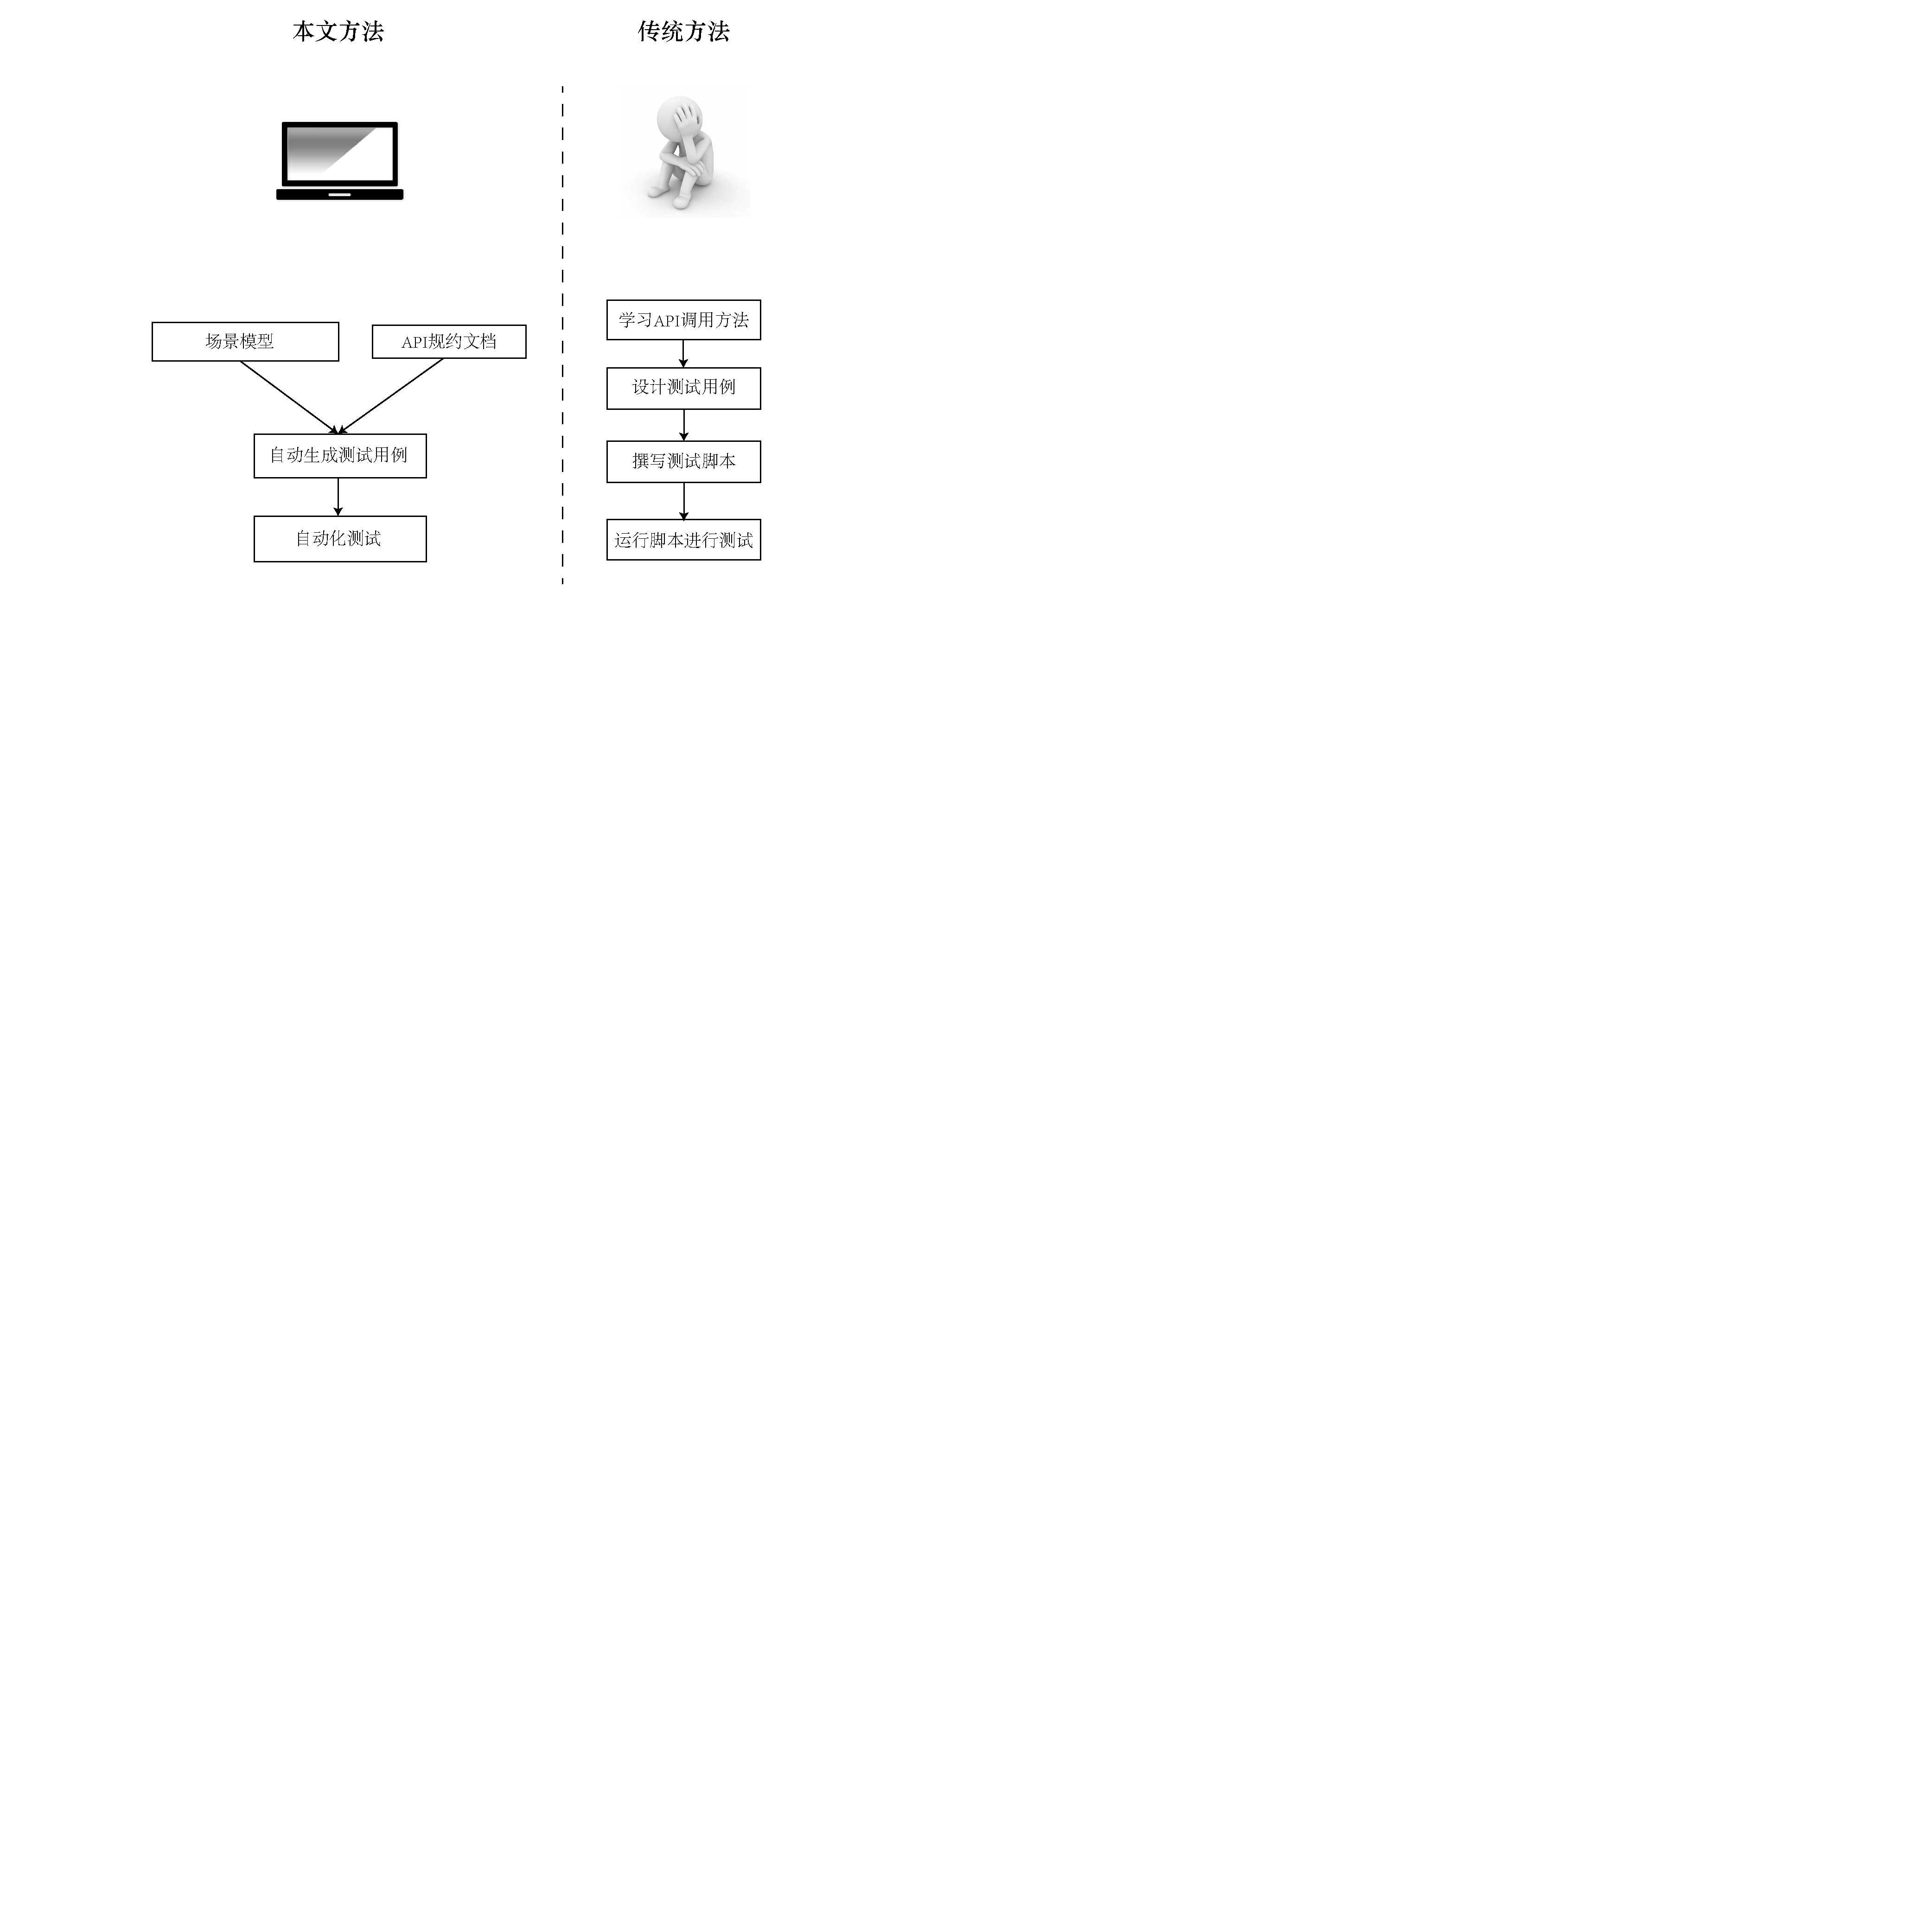
\includegraphics[width=300pt]{work_role_partial.pdf}
            \caption{本文方法与传统方法的对比. 在本文的方法中, 由于API规约文档已经提供, 人工参与的部分仅有场景设计, 其余部分均完全自动化. 而在传统方法中, API调用方法的学习, 测试用例的设计, 以及测试脚本的编写等, 均需要大量人力付出.}
            \label{fig:overview}
        \end{figure}
        
        图\ref{fig:overview}展示了本文提出的自动化测试方法的总体框架, 并将其与传统人工方法进行了对比. 如图中右半部分所示, 在传统方法中, 人工测试员首先需要学习API的调用请求方法, 然后设计测试用例, 编写测试脚本, 并手动运行测试脚本. 这个过程需要大量的人力付出, 并且冗长无聊, 耗时耗力. 此外, 测试的质量还很大程度上依赖于测试员的经验和水平.
        
        为了应对这些困难, 本文提出了一种自动化测试方法, 并实现了原型工具Lapis. 本文的自动化方法旨在以下方面改进传统方法:
        \begin{itemize}
            \item 测试设计. \\
                在本文的方法中, 测试人员只需要设计使用场景, 而不再是具体的每个测试用例. 本文的场景模型可以有效描述web API的控制流与数据流约束, 测试断言以及频繁使用模式. 相比直接设计测试用例, 由于一个测试场景可以自动生成多种各不相同的测试用例, 因此同样测试需求下, 所需场景数目少, 故设计测试场景可有效节约设计时间.
            
            \item 测试生成.\\
                在本文的方法中, 测试用例是由场景模型直接生成的. 使用本文提出的多种模块化测试数据生成算法和API调用序列生成算法, 测试用例的质量可以很容易地得到保证和提高. 并且, 由于实现了自动化, 测试用例的数量也可以远远超过手动设计的数量.
            
            \item 测试执行.\\
                目前已有的规约语言, 如OpenAPI, 提供了对RESTful API行为的详细形式化定义. 定义的组件包括了调用协议, 主机地址, 各个参数的格式和响应体的格式等等. 因此, 一旦有了测试数据, 便可以实现自动发送请求和响应解析.  本文实现了基于OpenAPI规约语言的工具原型, 可将人工测试员从书写API调用脚本的繁重劳动中解放出来.
        \end{itemize}
        本文介绍的原型工具Lapis, 即实现了此自动化方法, 该工具实现了包括规约导向的API分析, 使用场景模型解析, 测试用例生成和测试用例执行等功能.
        
        本文的结构安排如下: 第二章介绍基本模型与方法, 包括形式化的场景模型, 和基于模型的测试数据与测试用例生成方法. 第三章介绍原型系统的设计与实现, 包括原型系统的整体概述, 方法的具体实现等. 第四章展示原型系统在实际API服务上的实验结果, 并对实验结果进行了初步分析. 第五章进行总结, 并讨论了未来可继续进行的研究方向.
        
        % extended version
        % 本文的结构安排如下: 第二章介绍基本模型与方法, 包括形式化的场景模型, 和基于模型的测试数据与测试用例生成方法, 以及如何对生成的测试场景进行以故障检测为导向的优化. 第三章介绍原型系统的设计与实现, 包括原型系统的整体概述, 方法的具体实现等. 第四章展示原型系统在实际API服务上的实验结果, 并进行了实验结果的初步分析. 第五章进行总结, 并讨论了未来可继续进行的研究方向.
        


\chapter{场景建模与测试生成方法}
    \section{场景模型定义}
        \textbf{使用场景模型}是一种有效的模型化技术. 使用场景模型可以描述在现实世界中, 一或多个人如何与系统进行交互\footnote{http://agilemodeling.com/artifacts/usageScenario.htm}. 模型包括了交互过程中的步骤, 事件和动作. 本文提出了一种描述与web API的交互的使用场景模型. 为了基于模型进行测试生成, 模型着重于抽象以下web API的特点:
        
        \begin{itemize}
            \item 与使用场景相关的服务的元素. 这包括服务的功能, 请求数据, 响应数据, 执行约束等.
            
            \item 交互中, 各服务之间的交互. 这包括执行序列和序列内通信, 比如调用序列中之前某个服务的响应, 可能作为之后调用其他服务的参数.
            
            \item 不同交互操作的频率. 在有限测试资源的情况下, 对于测试资源的分配, 各个被测API需要有优先级顺序. 比如, 一些API可能在许多场景下都被用到, 被频繁地调用, 或者为许多其他API提供前置服务. 那么, 根据基于使用的测试原则, 这些频繁使用的API需要进行更多测试. 因此, 对API使用的分析与建模有助于优化对各个API和场景所生成的测试用例数量.
        \end{itemize}
        
        概率有限状态自动机(PFSA)可以有效描述相关服务, 执行序列和交互频率. 然而, 对于数据约束和服务通信, 它的能力有所不足. 我们的模型基于概率有限状态自动机进行扩展, 克服了这些不足.
        
        \subsection{背景: 概率有限状态自动机}
        
            概率有限状态自动机(PFSA)是非确定性有限状态自动机(NFA)的扩展. 它对非确定性有限状态自动机的转移, 起始状态和终止状态加入了概率因素. 对于每个串中读入的字符, 自动机会根据从当前状态出发的转移边的概率分布, 来从可选的转移边中选择一项进行转移. 状态的初始化和终止也具有类似的概率性质.
            
            根据Enrique Vidal等人的阐述\cite{enriquev05}, 一个基本的概率有限状态自动机具有如下的定义(定义\ref{def.pfsa}).
            
            \begin{definition}
                \label{def.pfsa}
                概率有限状态自动机为一个元组
                \begin{equation}
                    \mathcal{B} := <Q_{\mathcal{B}}, \Sigma, \sigma_{\mathcal{B}}, I_{\mathcal{B}}, F_{\mathcal{B}}, P_{\mathcal{B}}>,
                \end{equation}
                
                其中:
                \begin{itemize}
                    \item $Q_{\mathcal{B}}$是有限的状态集合;
                    
                    \item $\Sigma$是字符集;
                    
                    \item $\sigma_{\mathcal{B}} \subseteq Q_{\mathcal{B}} \times \Sigma \times Q_{\mathcal{B}}$是状态转移的集合;
                    
                    \item $I_{\mathcal{B}} : Q_{\mathcal{B}} \to \mathbb{R}^{+}$是各个状态作为起始状态的概率分布;
                    
                    \item $F_{\mathcal{B}}: Q_{\mathcal{B}} \to \mathbb{R}^{+}$是于各个状态处终止的概率分布;
                    
                    \item $P_{\mathcal{B}} : \sigma_{\mathcal{B}} \to \mathbb{R}^{+}$是各个转移边的转移概率.
                \end{itemize}
                
                $I_{\mathcal{B}}$函数满足初始状态概率归一化性质:
                \begin{equation}
                    \sum_{q \in Q_{\mathcal{B}}} I_{\mathcal{B}}(q) = 1.
                \end{equation}
                
                $F_{\mathcal{B}}$和$P_{\mathcal{B}}$函数满足转移概率归一化性质:
                \begin{equation}
                    \forall q \in Q_{\mathcal{B}}, \forall a \in \Sigma, F_{\mathcal{B}}(q) + \sum_{q' \in Q_{\mathcal{B}}} P_{\mathcal{B}}(q,a,q') = 1.
                \end{equation}
            \end{definition}
            
            按照惯例, 概率有限状态自动机使用带标签边的有向图表示. 图\ref{fig:PFSA_example}展示了一个概率有限状态自动机的例子. 其中, 图的节点表示自动机的状态, 图的带标签边表示自动机的概率转移边, 图的节点数字表示自动机状态的终止概率.
            
            \begin{figure}
                \centering
                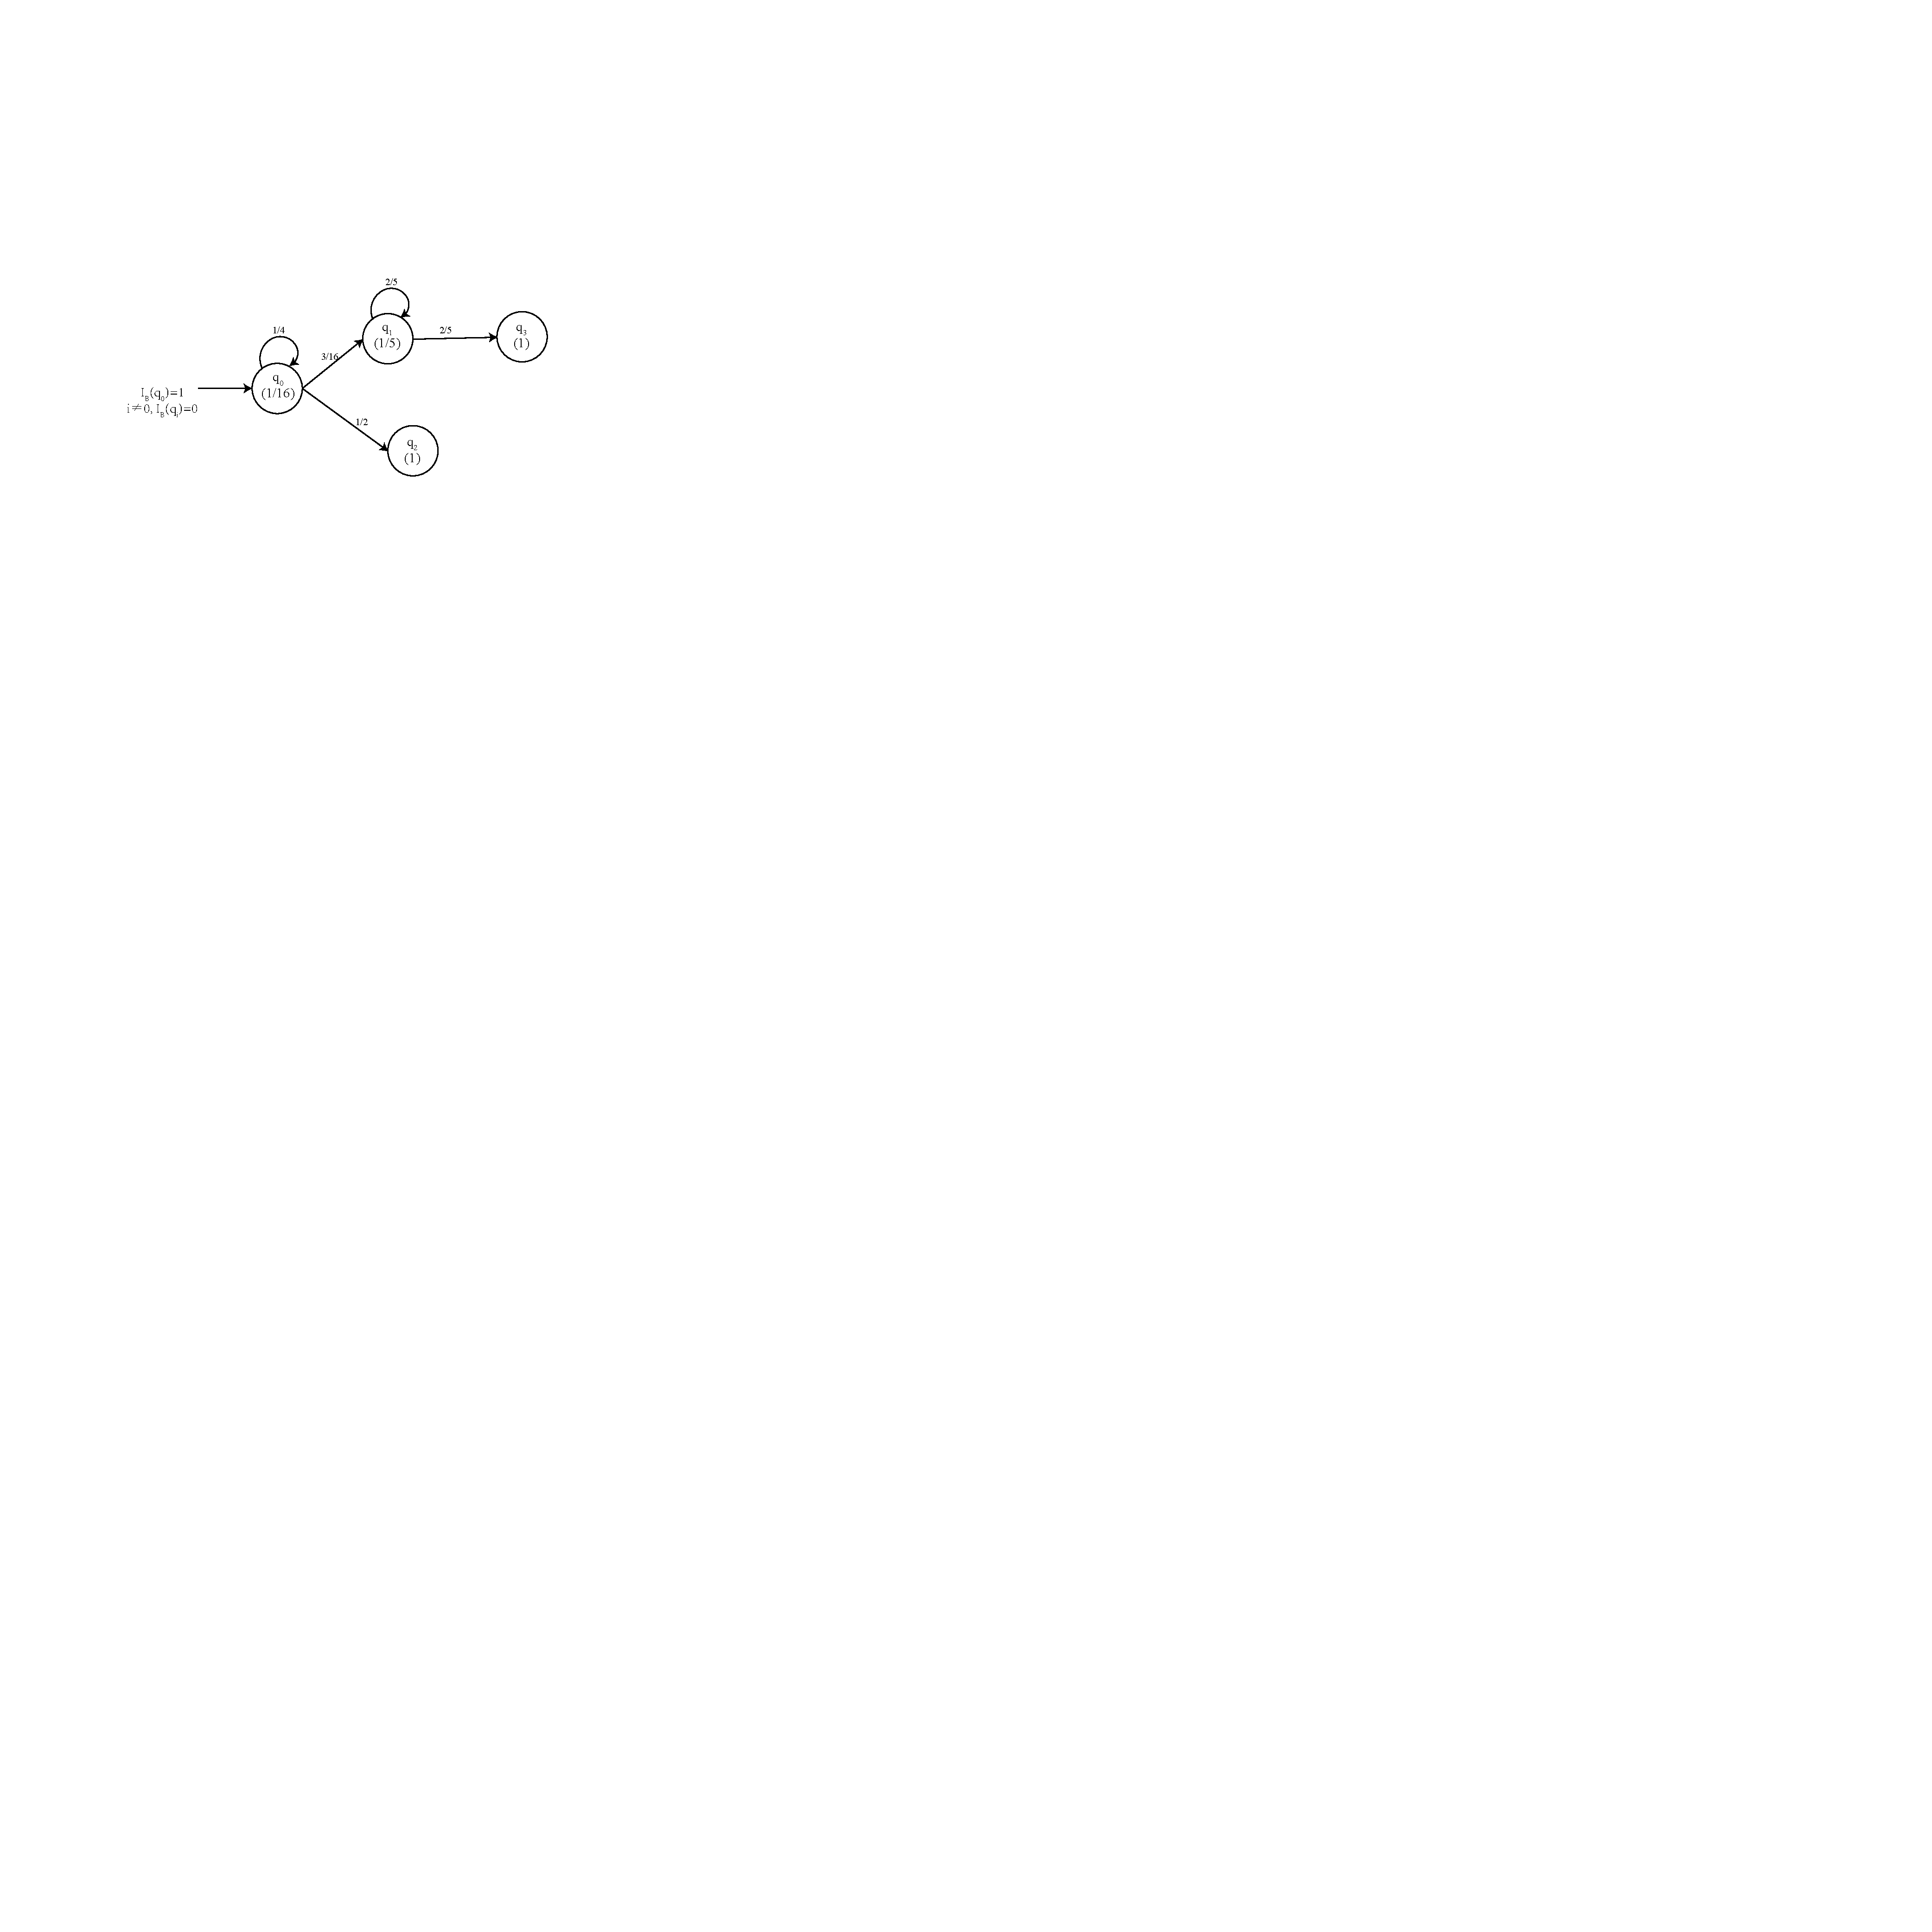
\includegraphics[width=300pt]{PFSA_example.pdf}
                \caption{概率有限状态自动机的可视化表示}
                \label{fig:PFSA_example}
            \end{figure}
            
            概率有限状态自动机是一种随机模型, 它生成的是在有限串集合$\Sigma^{*}$上的概率空间. 对于此自动机, 生成一个串的步骤为:
            
            \begin{itemize}
                \item 初始化: 按照概率分布$I_\mathcal{B}$选择一个$Q_{\mathcal{B}}$中的状态$q_0$作为初始状态;
                
                \item 生成: $q$表示当前状态, $a$表示当前读入字符. 则以$F_{\mathcal{B}}(q)$的概率决定是否在此状态处终止, 或者以$P_{\mathcal{B}}(q, a, q')$的概率决定是否进行转移$(q,a,q')$. 如果进行此转移, 则将$q'$置为当前状态.
            \end{itemize}
        
            概率有限状态自动机的以下特点让其适用于使用场景的建模:
            
            \begin{itemize}
                \item 自动机的状态可以很方便地与服务端点关联起来. 因此, 状态的转移可对执行序列进行建模.
                
                \item 自动机的字符集$\Sigma$可建模服务端点的所有可能的响应. 另一方面, 每个状态转移均对应一个字符$c \in \Sigma$, 其表示此转移仅适用于当前读入字符为$c$的情形. 因此, 这个对应字符可建模各个转移所适用的范围, 此范围由服务端点的返回响应决定. 也就是状态转移对应的字符定义了进行此状态转移的条件.
                
                \item 自动机的起始概率, 终止概率, 转移概率反映了进行不同交互的频率差异.
            \end{itemize}
            
            然而, 在使用场景模型中关键的数据约束, 数据依赖, 测试断言则很难在概率有限状态自动机中表达与反映. 本文的场景模型扩展了概率有限状态自动机模型来克服这些问题.
        
        \subsection{形式化定义}
            本文的场景模型在以下方面扩展了基本的概率有限状态自动机:
            
            \begin{itemize}
                \item 它在状态定义中加入了请求数据约束与请求数据依赖的定义, 以便于生成请求数据.
                
                \item 它在状态定义中加入了响应数据约束与测试断言 的定义, 以便于对响应进行验证.
            \end{itemize}
            
            形式化的定义如下:
            
            \begin{definition}
                \label{def:our}
                场景模型是一个元组
                \begin{equation}
                     \mathcal{A} := <Q_{\mathcal{A}}, \Sigma, \sigma_{\mathcal{A}}, I_{\mathcal{A}}, F_{\mathcal{A}}, P_{\mathcal{A}}>,
                \end{equation}
                
                其中:
                \begin{itemize}
                    \item $Q_{\mathcal{A}}$是有限的状态集合;
                    
                    \item $\Sigma$是所有可能的API响应的集合;
                    
                    \item $\sigma_{\mathcal{A}} \subseteq Q_{\mathcal{A}} \times \Sigma \times Q_{\mathcal{A}}$是状态转移的集合;
                    
                    \item $I_{\mathcal{A}} : Q_{\mathcal{A}} \to \mathbb{R}^{+}$是各个状态作为起始状态的概率分布;
                    
                    \item $F_{\mathcal{A}} : Q_{\mathcal{A}} \to \mathbb{R}^{+}$是于各个状态处终止的概率分布;
                    
                    \item $P_{\mathcal{A}}: \sigma_{\mathcal{A}} \to \mathbb{R}^{+}$是各个转移边的转移概率.
                \end{itemize}
                
                对于$I_{\mathcal{A}}$, $F_{\mathcal{A}}$, $P_{\mathcal{A}}$, 仍然要求满足归一化性质:
                \begin{equation}
                    \sum_{q \in Q_{\mathcal{A}}} I_{\mathcal{A}}(q) = 1;
                \end{equation}
                与
                \begin{equation}
                    \forall q \in Q_{\mathcal{A}}, \forall a \in \Sigma, F_{\mathcal{A}}(q) + \sum_{q' \in Q_{\mathcal{A}}} P_{\mathcal{A}}(q,a,q') = 1.
                \end{equation}
                
                状态$q \in Q_{\mathcal{A}}$的定义是一个元组
                \begin{equation}
                    q := <t_q, in_q, out_q, d_q, a_q>,
                \end{equation}
                其中:
                \begin{itemize}
                    \item $t_q$可以为$empty$(表示不与API服务端点关联)或一个服务端点的名称;
                    
                    \item $in_q$是所有合法请求数据的集合;
                    
                    \item $out_q$是所有合法响应体的集合;
                    
                    \item $d_q$是请求数据依赖的集合;
                    
                    \item $a_q$是对响应体的断言的集合.
                \end{itemize}
                
                作为所有可能的API的响应的集合, $\Sigma$满足
                \begin{equation}
                    \Sigma = \bigcup_{q \in Q_{\mathcal{A}}} out_q.
                \end{equation}
                
                在状态$q$的定义中, 每一项请求数据依赖$d \in d_q$都是一个元组
                \begin{equation}
                    d := <q_d, index_d, f_d>,
                \end{equation}
                它的各项含义为:
                \begin{itemize}
                    \item $q_d \subseteq Q_{\mathcal{A}}$是场景模型$\mathcal{A}$中的一个或多个状态的集合;
                    
                    \item $index_d \in \mathbb{Z}$是一个整数;
                    
                    \item $f_d: \bigcup_{q' \in q_d} in_{q'} \times out_{q'} \to i \subseteq in_q$是一个函数, 此函数定义了给定状态$q_d$上的请求数据和得到的响应时, 对当前状态$q$而言, 合法的请求数据集合.
                \end{itemize}
                
                在状态$q$的定义中, 每一项响应体的断言$a \in a_q$也是一个元组
                \begin{equation}
                    a := <q_a, index_a, f_a>,
                \end{equation}
                它的各项含义为:
                \begin{itemize}
                    \item $q_a \subseteq Q_{\mathcal{A}}$是场景模型$\mathcal{A}$中的一个或多个状态的集合;
                    
                    \item $index_a \in \mathbb{Z}$是一个整数;
                    
                    \item $f_a: \bigcup_{q' \in q_a} in_{q'} \times out_{q'} \to o \subseteq out_q$是一个函数, 此函数定义了给定状态$q_a$上的请求数据和得到的响应时, 对当前状态$q$而言, 合法的响应数据集合.
                \end{itemize}
            \end{definition}
            
            需要注意的是, 在web API测试的语义下, 输入数据是测试方法所生成的, 也就是对某个API服务端点的请求数据. 输出数据则是API返回的响应体.
        
        \subsection{解释与说明}
            在本文的场景模型中, 对输入数据的约束集合$in_q$附带在每个状态$q$里. 输入数据的约束集合定义了输入数据的取值空间, 即满足所有约束的数据构成了输入数据的取值空间, 数据的生成就是为此取值空间赋予概率分布, 然后进行随机采样. 对输出数据的约束集合$out_q$也附带在每个状态$q$里, 使用输入数据请求对应API服务端点, 得到的响应使用约束条件进行验证, 便可以检验API的行为是否符合定义.
            
            而输入数据的依赖$d := <q_d, index_d, f_d >$则表达了由上下文对当前状态赋予的请求数据的额外约束. 其具体含义为: 在模型上遍历的同时记录下当前的状态序列, 然后保序提取出属于$q_d$的状态, 找出其中的第$index_d$项状态(下标$index_d$从0开始, 负数表示倒数$|index_d|$个状态). 此时, $(q_d, index_d)$指向了当前状态序列中某一个确定元素$now$. 然后, 提取出该状态执行时的请求数据(即输入, 记为$i_{now}$)与响应(即输出, 记为$o_{now}$), 再应用到函数$f_d$, 得到的$f_d(i_{now}, o_{now})$定义了更严格的合法的当前请求数据(即当前输入)集合. 可以看出, 合法输入数据的集合由当前执行状态序列中之前的输入输出决定.
            
            响应体的断言$a := <q_a, index_a, f_a>$的具体含义也相似. 这里, $f_a(i_{now}, o_{now})$定义的是更严格的合法的当前响应(即当前输出)集合.
            
            $f_d$和$f_a$函数虽然取上下文中之前的输入和输出数据作为参数, 但也可以不依赖于这两项, 此时, 则相当于直接对当前状态施加额外的输入数据限制和输出断言, 作用与$in_q$和$out_q$相似. 不过, 在具体实现时, $in_q$和$out_q$是由API规约文档引入的, 而$f_d$和$f_a$包含在场景模型内.
        
        \subsection{示例}
            \begin{figure}
                \centering
                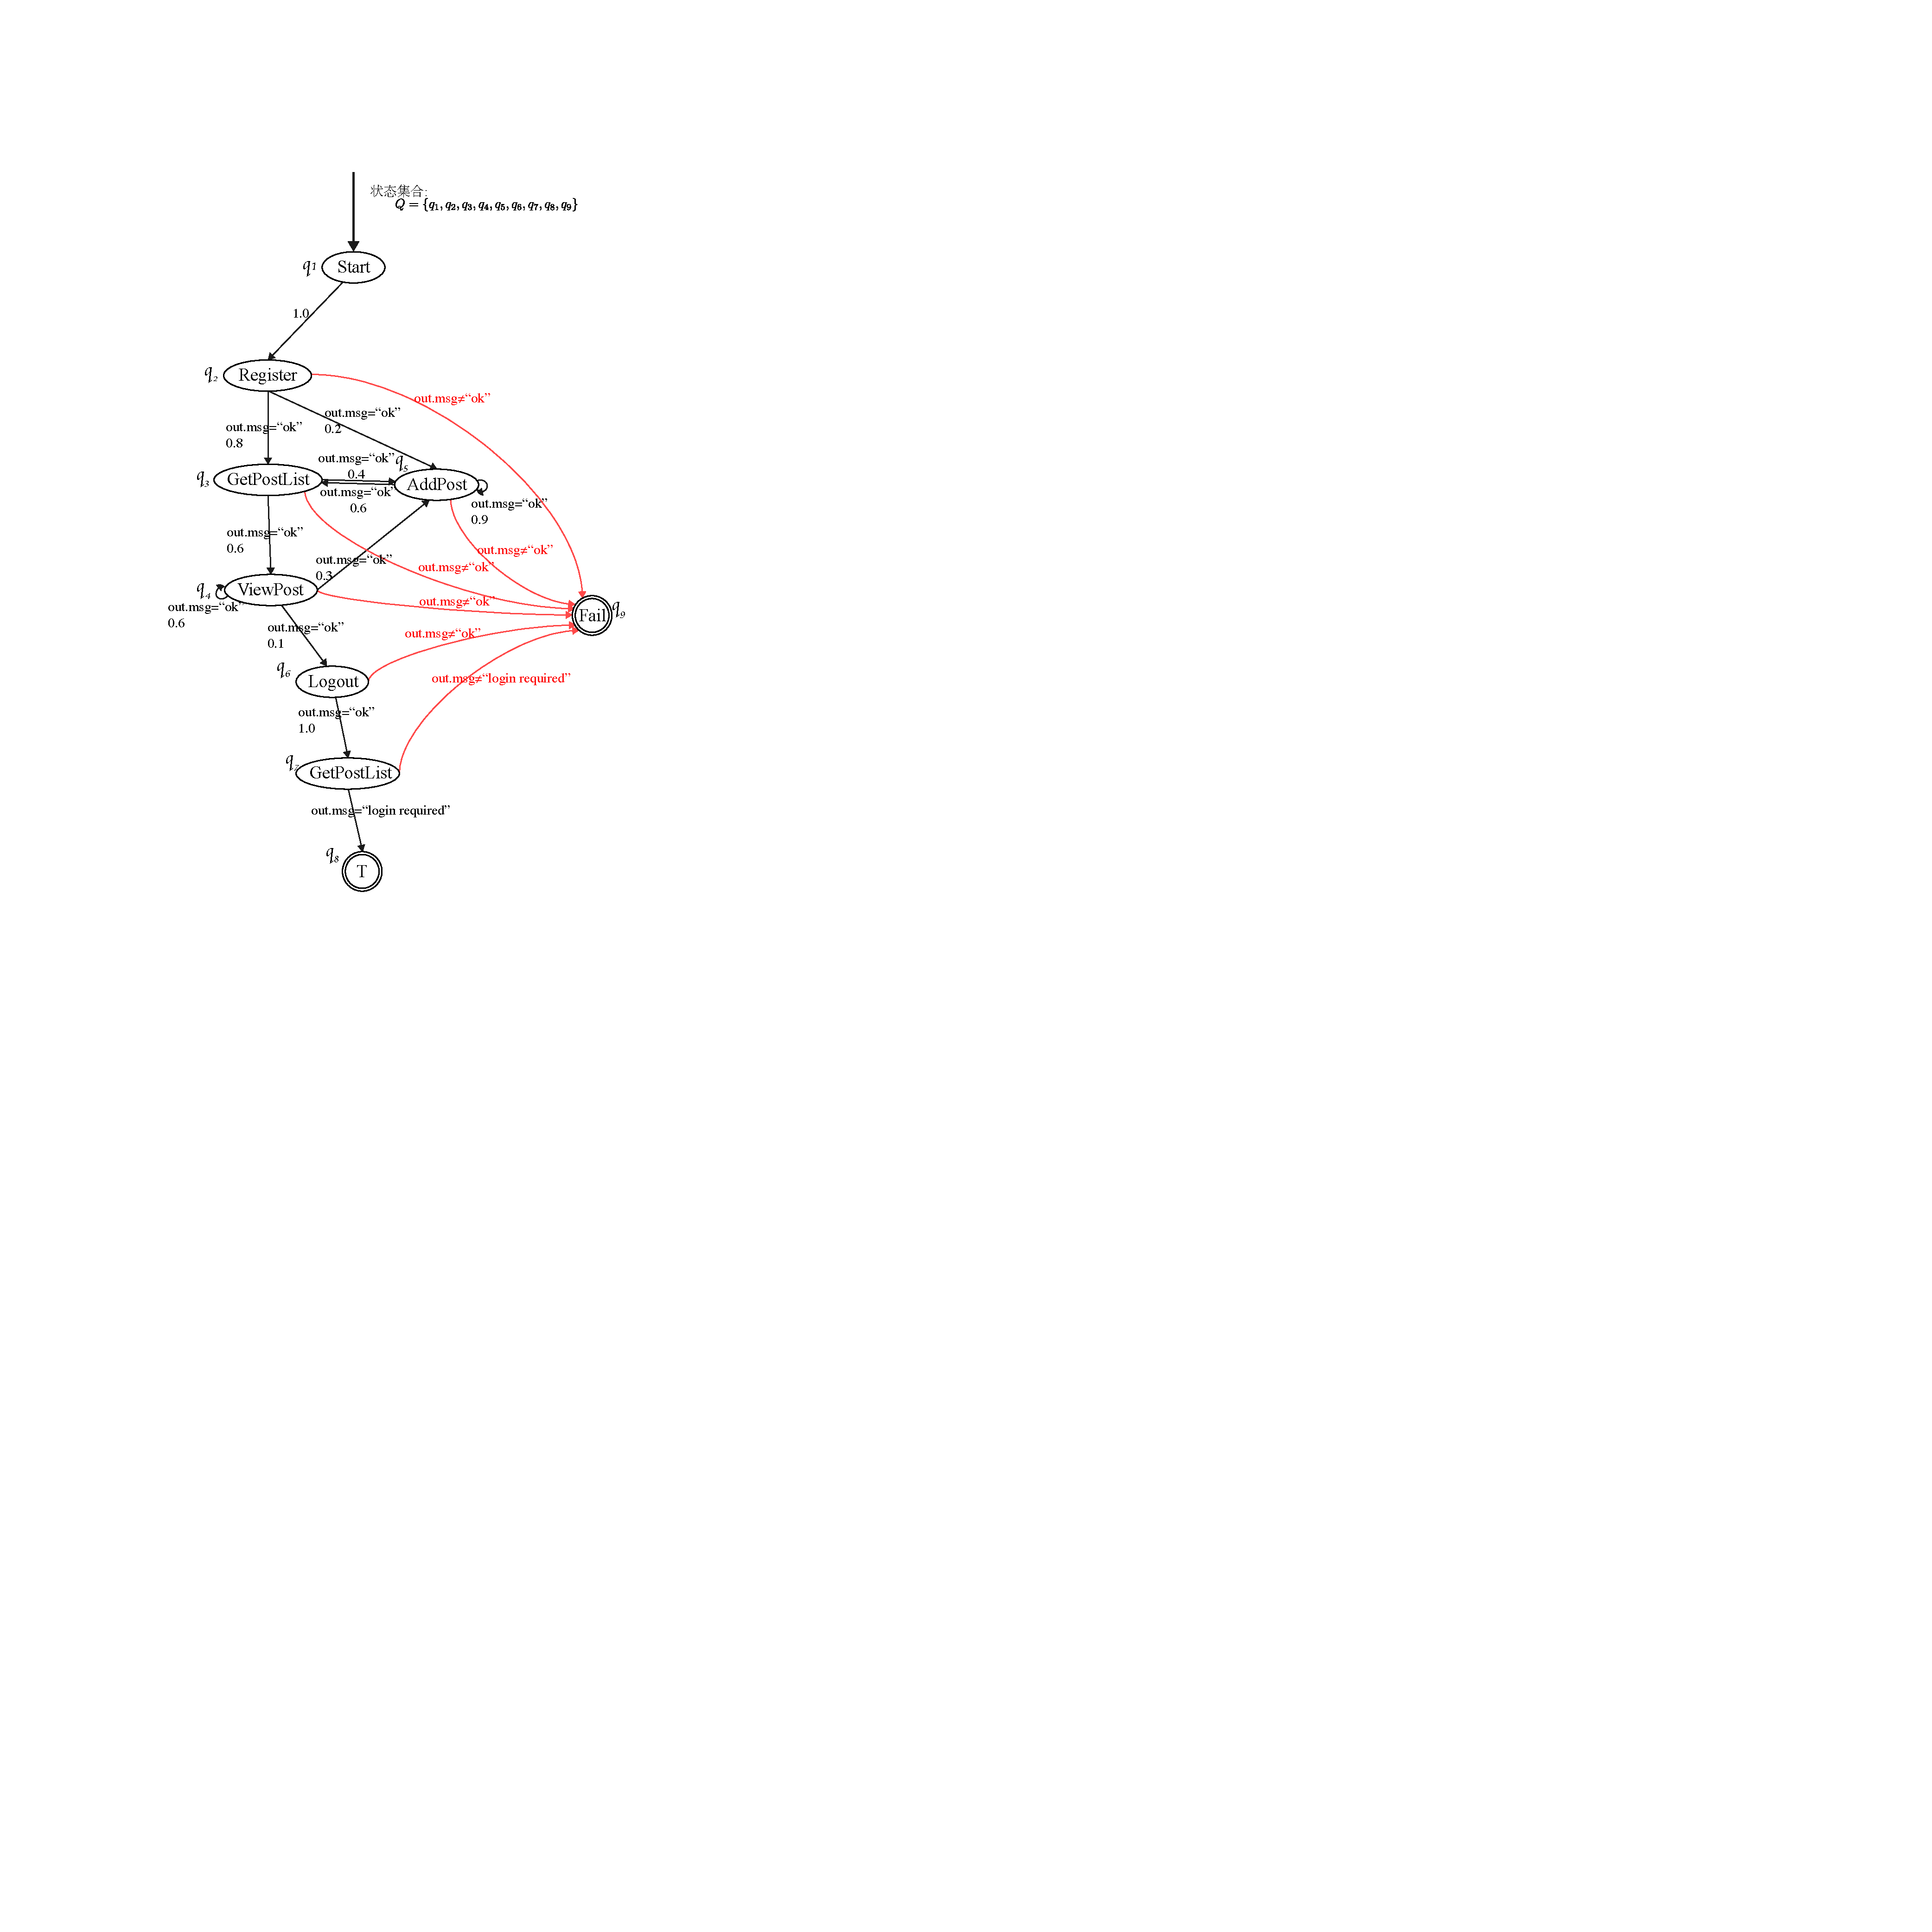
\includegraphics[width=300pt]{scenario_example.pdf}
                \caption{一个场景模型的实例. 输入数据依赖和响应体断言为: \\
                $q_3$.\texttt{request.username} = $q_2$.\texttt{request.username};\\
                $q_3$.\texttt{request.ssid} = $q_2$.\texttt{response.ssid};\\
                $q_4$.\texttt{request.username} = $q_2$.\texttt{request.username};\\
                $q_4$.\texttt{request.postId} = $q_3$.\texttt{response.posts}.\\
                这里省略了下标的定义, 状态集合的定义($q_d$, $q_a$)和函数的定义($f_d$, $f_a$)以谓词形式给出.}
                \label{fig:scenario_example}
            \end{figure}
            
            图\ref{fig:scenario_example}为一个典型的场景模型的示例. 这个场景模型是为一个类似微博的自媒体平台服务设计的. 在这个服务里, 用户可以登录, 浏览微博, 发布新微博. 服务开发的5个API接口为: “Register”(注册)、“GetPostList”(获取动态)、“ViewPost”(浏览微博)、“AddPost”(发布)、“Logout”(登出). 在图中, 类似自动机的表示方法, 使用图的节点来表示场景模型的状态, 使用图的边表示场景模型的转移, 边上的数字表示转移概率, 边上的文字表示转移条件. 示例中共有9个状态和18项转移. 初始状态只有一个, 为$q_1$(“Start”). 终止状态有两个, 为$q_8$和$q_9$(“T”和“Fail”). 这里的初始状态和终止状态是确定性的($I(\cdot) \in {0,1}$, $F(\cdot) \in {0,1}$), 但场景模型也支持概率性的. 除了初始状态和终止状态, 示例中其他的状态均与API服务端点关联, 图中对应节点上的标签即为关联API的名称. 处于这些状态时, 就会向这些对应API发送请求. 举例来说, $q_2$对应注册API, $q_3$对应获取动态API. 在转移边上, 概率的不相等可以反映出实际使用场景下, 不同执行路径的频率的不相等.
        
        \subsection{构建与实现}
            场景模型抽象了API的使用场景, 并为生成高效的测试用例提供了必需的只是. 目前, 场景模型需要手工进行构建与设计, 然后才能自动生成与执行测试用例. 未来, 将进一步探索如何从自然语言描述和日志文件中进行自动化场景生成.
            
            场景模型使用与OpenAPI规范类似的YAML格式描述. 在本文的工具中, 使用OpenAPI的脚本描述相关API, 使用场景模型描述使用场景, 两者共同作为工具的输入. 生成的测试用例及其执行结果则是工具的输出.
            
            在具体实现上, 合法输入(包括输入依赖), 合法响应(包括输出断言), 转移条件的定义($in_q$, $out_q$, $f_d$, $f_a$, $x \in Sigma$)的定义有多种来源:
            
            \label{sec:set_define}
            \begin{itemize}
                \item JSON模式(JSON Schema)\footnote{https://tools.ietf.org/html/draft-wright-json-schema-validation-00}. JSON模式被用于结构化JSON数据的验证. 对于一个JSON模式定义而言, 通过验证的数据构成了一个固定集合. 当所需集合不依赖于其他状态(即上下文)时, 便可以使用JSON模式定义. 因此, 对于输入依赖和输出断言的定义, 由于需要定义依赖上下文的函数($f_d$, $f_a$), 一般不使用JSON模式定义. 在使用OpenAPI描述的API脚本文档中, 均采用这种方法描述合法输入和合法响应. 场景模型中的状态定义如果关联了一个API服务端点, 则默认将此API的脚本文档中的合法输入, 合法响应的定义作为$in_q$和$out_q$.
                
                \item 自定义校验函数. 本文的工具支持可扩展插件. 用户可以编写并引入校验函数, 校验函数接受数据作为输入, 判定数据是否满足条件. 因此, 满足条件的数据构成了一个集合. 这种定义方式只能在合法响应(包括输出断言)和转移条件的定义中使用, 因为定义合法输入时还需要在定义的集合中采样, 而只判定是否属于某集合的函数显然不具备此功能.
                
                \item 自定义生成函数. 用户可以编写并引入生成函数, 生成函数要求随机返回一个在其隐式定义的集合内的元素. 因此, 它并不能判定某个数据是否属于其定义的集合, 也不能获取其定义集合的所有元素. 所以, 它只能用于定义合法输入(包括输入依赖), 这是因为测试时只需要一定随机地获得满足条件的数据(即采样集合内的元素)即可, 而不需要知道整个集合. 它不能用于定义合法响应和转移条件.
            \end{itemize}
            
    
    \section{测试生成方法}
        现在, 有了OpenAPI格式的API行为描述文档, 和场景模型, 接下来的任务就是生成并执行测试了. 测试的生成有两个层次: 一个是为单次API请求生成请求数据(即输入数据), 一个是将单个请求串联起来生成API执行序列作为测试用例.
        
        \subsection{请求数据生成}
            请求数据的生成, 就是在合法请求数据集合中的随机采样. \ref{sec:set_define}小节总结了目前支持的集合定义方法: 在定义合法输入时, 有JSON模式和自定义生成函数两种定义方法.
            
            当合法输入使用JSON模式定义时, 由于每个数据结构都属于JSON模式定义的基本类型之一, 因此, 本文分类讨论, 为每个基本类型设计了缺省采样策略. 对于一些特殊子类型如日期、时间、二进制串等, 还定义了特殊采样策略. 具体策略见表\ref{tab:schemagen}. 特别地, 当多个条件均满足时, 则合理结合多个策略生成.
            
            \begin{table}[]
                \centering
                \begin{tabular}{rll}
                    \toprule
                    类型 & 条件 & 策略 \\
                    \midrule
                    null & / & 返回元素\texttt{Null} \\
                    \hline
                    integer \& & 存在\texttt{multipleOf}域 & 从满足倍数关系的值空间中采样 \\
                    \cline{2-3}
                    float & 存在\texttt{enum}域 & 从定义的有限集合中采样 \\
                    \cline{2-3}
                    & 存在\texttt{MIN}或\texttt{MAX}域 & 从定义的区间中采样 \\
                    \cline{2-3}
                    & / & 在对应类型的整个区间中采样 \\
                    \hline
                    boolean & 存在\texttt{enum}域 & 从定义的有限集合中采样 \\
                    \cline{2-3}
                    & / & 使用伯努利分布($p=0.5$) \\
                    \hline
                    string & 存在\texttt{regex}域 & 从正则表达式定义的模式中生成 \\
                    \cline{2-3}
                    & 存在\texttt{enum}域 & 从定义的有限集合中采样 \\
                    \cline{2-3}
                    & \multirow{2}{*}{\texttt{format}域存在且为\texttt{'date'}} & 先随机日期, \\
                    & & 再以RFC3339的full-date格式表示 \\
                    \cline{2-3}
                    & \multirow{2}{*}{\texttt{format}域存在且为\texttt{'datetime'}} & 先随机日期时间, \\
                    & & 再以RFC3339的date-time格式表示 \\
                    \cline{2-3}
                    & \texttt{format}域存在且为\texttt{'binary'} & 随机二进制串, 以\texttt{bytes}格式返回 \\
                    \cline{2-3}
                    & \multirow{2}{*}{存在\texttt{minLength}或\texttt{maxLength}域} & 先从指定长度区间随机长度值, \\
                    & & 再随机生成字符串 \\
                    \cline{2-3}
                    & \multirow{2}{*}{/} & 先随机确定长度值(默认不超过255),\\
                    & & 再随机生成字符串 \\
                    \hline
                    array & \multirow{2}{*}{存在\texttt{maxItems}或\texttt{minItems}域} & 先从指定区间随机列表长度,\\
                    & & 再随机递归生成各元素 \\
                    \cline{2-3}
                    & \multirow{2}{*}{/} & 先随机确定列表长度,\\
                    & & 再随机递归生成各元素 \\
                    \hline
                    object & / & 递归生成各成员 \\
                    \bottomrule
                \end{tabular}
                \caption{从JSON模式生成请求数据. 依据基本类型和条件分类讨论, 采取不同策略.}
                \label{tab:schemagen}
            \end{table}
            
            当合法输入使用自定义生成函数定义时, 由于函数期望的返回值就是其隐式定义的集合的采样, 故直接将返回值作为请求数据即可.
        
        \subsection{执行序列生成}
            如果以自动机的视角审视场景模型, 那么它所定义的仍然是合法串的集合以及它们的概率分布. 由于每个自动机的状态可以与一个API服务端点关联, 所以产生的串也可以对应于API的请求/执行序列. 在进行web API测试时, 一个这样的包含具体请求数据的序列, 即是一个测试用例.
            
            因此, 执行序列生成算法的基本思想, 就是根据场景模型定义的概率分布生成可以被其接受的串. 相比看似相近的概率图模型和马尔科夫模型, 场景模型中转移到某一状态不仅仅由当前状态和概率分布决定. 由于每项转移是否可用取决于关联的API服务端点的响应结果, 而API服务端点的响应结果取决于输入的请求数据, 请求数据的生成过程依赖整个当前序列, 故状态转移还可以与之前的所有状态均相关. 因此, 场景模型的表达能力要强于仅与当前状态和概率分布相关的概率图模型与马尔科夫模型.
            
            执行序列生成算法的大体流程如算法\ref{algo:seqgen}所示.
            
            在算法\ref{algo:seqgen}中, 首先, 根据初始状态概率分布函数$I_{\mathcal{A}}$随机选择初始状态. \texttt{RandomChoice()}函数接受两个列表作为参数, 分别表示候选元素和每个元素的概率权重, 它按照权重随机抽取一个元素作为返回值, 故\texttt{RandomChoice(}$Q_{\mathcal{A}}$\texttt{,}$I_{\mathcal{A}}$\texttt{)}返回随机选择的初始状态. 然后, 算法在自动机上进行遍历. 每一步中, 使用$current$记录当前所处状态, 请求数据和响应数据等上下文信息. $r$是存储每一步的上下文信息的总列表. 如果当前状态与一个API服务端点相关联, 算法将遍历请求数据的各个参数定义, 并从数据依赖定义或合法集合定义中随机生成出参数. 之后, 算法发送请求并解析响应体. 解析完成后, 算法扫描响应的各个域, 根据断言定义或合法集合定义进行验证, 如果验证不通过, 算法终止. 最后, 算法根据终止概率分布函数$F_{\mathcal{A}}$进行概率终止, 若未终止, 则根据响应和转移概率函数$P_{\mathcal{A}}$随机选择下一状态, 进入下一步.
            
            当算法结束时, 返回的值包括执行序列$r$和终止原因$T$, 其中终止原因$T$详细记录了跳出算法循环的位置和具体信息, 便于发现被测系统故障时进行修复.
            
            从描述中可以看出, 算法结合了执行序列的生成和具体执行, 并且生成过程实时受执行反馈(即API响应)影响. 序列生成是动态的, 这使预处理相关的加速和优化变得困难, 但也使生成的序列更为灵活, 更为贴近实际使用场景.
            
            \begin{algorithm}
              	\scriptsize
              	
                \caption{API执行序列生成算法}
              	
                \KwIn{$Spec$, $\mathcal{A}$} 
                \tcp{输入: API定义脚本和场景模型脚本}
                \tcp{场景模型$\mathcal{A} := <Q_{\mathcal{A}}, \Sigma, \sigma_{\mathcal{A}}, I_{\mathcal{A}}, F_{\mathcal{A}}, P_{\mathcal{A}}>$}
                \KwOut{$r$, $T$}
                \tcp{输出: 执行序列和终止原因}
                $q$ $\gets$ RandomChoice($Q_{\mathcal{A}}$, $I_{\mathcal{A}}$)\;
                \tcp{根据初始状态概率分布函数随机初始状态$q := <t_q, in_q, out_q, d_q, a_q>$}
                $current$ $\gets$ $EmptyMap$\;
                $current.state$ $\gets$ $q$\;
                $r$ $\gets$ $EmptyList$\;
                $stop$ $\gets$ $false$\;
                \While {$\neg stop$} {
                	$i$ $\gets$ $EmptyMap$\;
                    $o$ $\gets$ $EmptyMap$\;
                	\If(\tcp*[h]{$q$有关联的API服务端点}) {$t_q \neq empty$}{
                    	\ForEach(\tcp*[h]{遍历处理所有请求参数}) {$param$ in $t_q.params$} {
                        	\If(\tcp*[h]{当前参数$param$有数据依赖, 则从依赖生成请求数据}) {$d_q.param \neq Null$} {
                            	$d$ $\gets$ $d_q.param$\;
                                \tcp{数据依赖$d := <q_d, index_d, f_d>$}
                                $q'$ $\gets$ PickDependee($r$, $q_d$, $index_d$)\;
                                $i.param$ $\gets$ RandomFromSet($f_d(i_{q'}, o_{q'})$)\;
                            } \Else(\tcp*[h]{当前参数$param$无数据依赖, 则默认从合法请求集合中生成请求数据}) {
                            	$i.param$ $\gets$ RandomFromSet($in_q.param$)\;
                            }
                        }
                        $o$ $\gets$ Request($Spec.t_q$, $i$)\;
                        \tcp{发送请求, 并解析返回的响应}
                        $current.i$ $\gets$ $i$\;
                        $current.o$ $\gets$ $o$\;
                        \If(\tcp*[h]{请求失败}) {RequestFail($o$)} {
                        	$T$ $\gets$ ``Request Fail''\;
                            $stop$ $\gets$ $true$\;
                        } \Else(\tcp*[h]{请求成功}) {
                        	\ForEach(\tcp*[h]{遍历返回的响应的各个域}) {$field$ in $Spec.t_q.fields$} {
                            	\If(\tcp*[h]{响应的$field$域有断言定义, 则验证是否满足断言}) {$a_q.field \neq Null$} {
                                	$a$ $\gets$ $a_q.field$\;
                                    \tcp{响应断言$a := <q_a, index_a, f_a>$}
                                    $q'$ $\gets$ PickDependee($r$, $q_a$, $index_a$)\;
                                    \If {$o.field \notin f_a(i_{q'}, o_{q'})$} {
                                    	$T$ $\gets$ ``Response Assert Fail''\;
                                        $stop$ $\gets$ $true$\;
                                    }
                                } \Else(\tcp*[h]{响应的$field$域无断言定义, 则默认直接验证是否是合法响应}) {
                                	\If {$o.field \notin out_q.field$} {
                                    	$T$ $\gets$ ``Response Illegal Fail''\;
                                        $stop$ $\gets$ $true$\;
                                    }
                                }
                            }
                        }
                    }
                    $r$.append($current$)\;
                    \If {$\neg stop$} {
                    	$\chi$ $\gets$ RandomNumber($U(0,1)$)\;
                        \If(\tcp*[h]{依照终止概率分布函数决定是否终止执行}) {$\chi \le F_{\mathcal{A}}(q)$} {
                        	$T$ $\gets$ ``Final State''\;
                            $stop$ $\gets$ $true$\;
                        }
                    }
                	\If(\tcp*[h]{继续执行, 依照转移概率分布函数选择转移边}) {$\neg stop$} {
                    	$q$ $\gets$ RandomChoice($\sigma_{\mathcal{A}}(q,o)$, $P_{\mathcal{A}}(q,o)$)\;
                        $current$ $\gets$ $EmptyMap$\;
                        $current.state$ $\gets$ $q$\;
                    }
                }
                \Return {$r$, $T$}
    
                \label{algo:seqgen}
              \end{algorithm}
        
        \subsection{启发式执行序列生成}
            除了以上提出的算法, 本文亦探索了启发式的执行序列生成. 启发式的改进主要在转移边的选择方面. 在以上算法中, 转移边的选择严格按照定义的概率权值, 然而, 在运行此算法多次以生成多个测试用例时, 为了提高测试覆盖率, 可以不必拘泥于定义的权值, 而加入一定的调整.
            
            在此场景模型中, 测试覆盖率常常与场景的状态覆盖率, 转移覆盖率, 以及综合路径覆盖率有正相关. 一个基本的思想便是将这些覆盖率的提升期望加入考虑, 对提升期望高的转移边增大选择概率.
            
            一种贪心策略是优先选择连接到未访问状态的转移边, 或直接选择未访问的转移边. 但是, 本文的实验发现, 由于场景模型目前采用人工设计, 包含的状态数和转移边数较少, 因此少量测试用例即可完全遍历, 故价值不大. 其他更复杂的转移很可能会有效, 如考虑连续状态序列或整体路径的覆盖率等, 这有待进一步实验证实.
            
            另一方面, 启发式改进的直接作用亦可能并不显著. 虽然不使用启发式算法时, 测试用例冗余度较高, 即单位用例覆盖率不够高. 但收益于全自动生成的过程, 同等时间下, 生成测试用例的数目很大, 这可在一定程度上弥补甚至逆转总覆盖率的劣势. 具体结论需要依据具体场景模型进行评估, 也是值得进一步探讨的问题.
    
    % extended version
    % \section{*启发式优化}
    %     \subsection{启发式执行序列生成}
    %     将上个小节移到本章来
    %     \subsection{启发式场景优化}
    %     不知道有冇时间做了


\chapter{原型系统设计与实现}

    原型系统包括核心工具Lapis和用户接口两大组件. 其中, 核心工具提供从脚本解析到测试生成与执行的整套方法的原型实现. 用户接口则包括核心工具的编程API接口, 在线API脚本的上传、编辑和可视化的web应用, 以及桌面端测试管理系统. 以上各部分完全独立.

	\section{核心工具Lapis}
	
	    \begin{figure}[!htb]
	        \centering
	        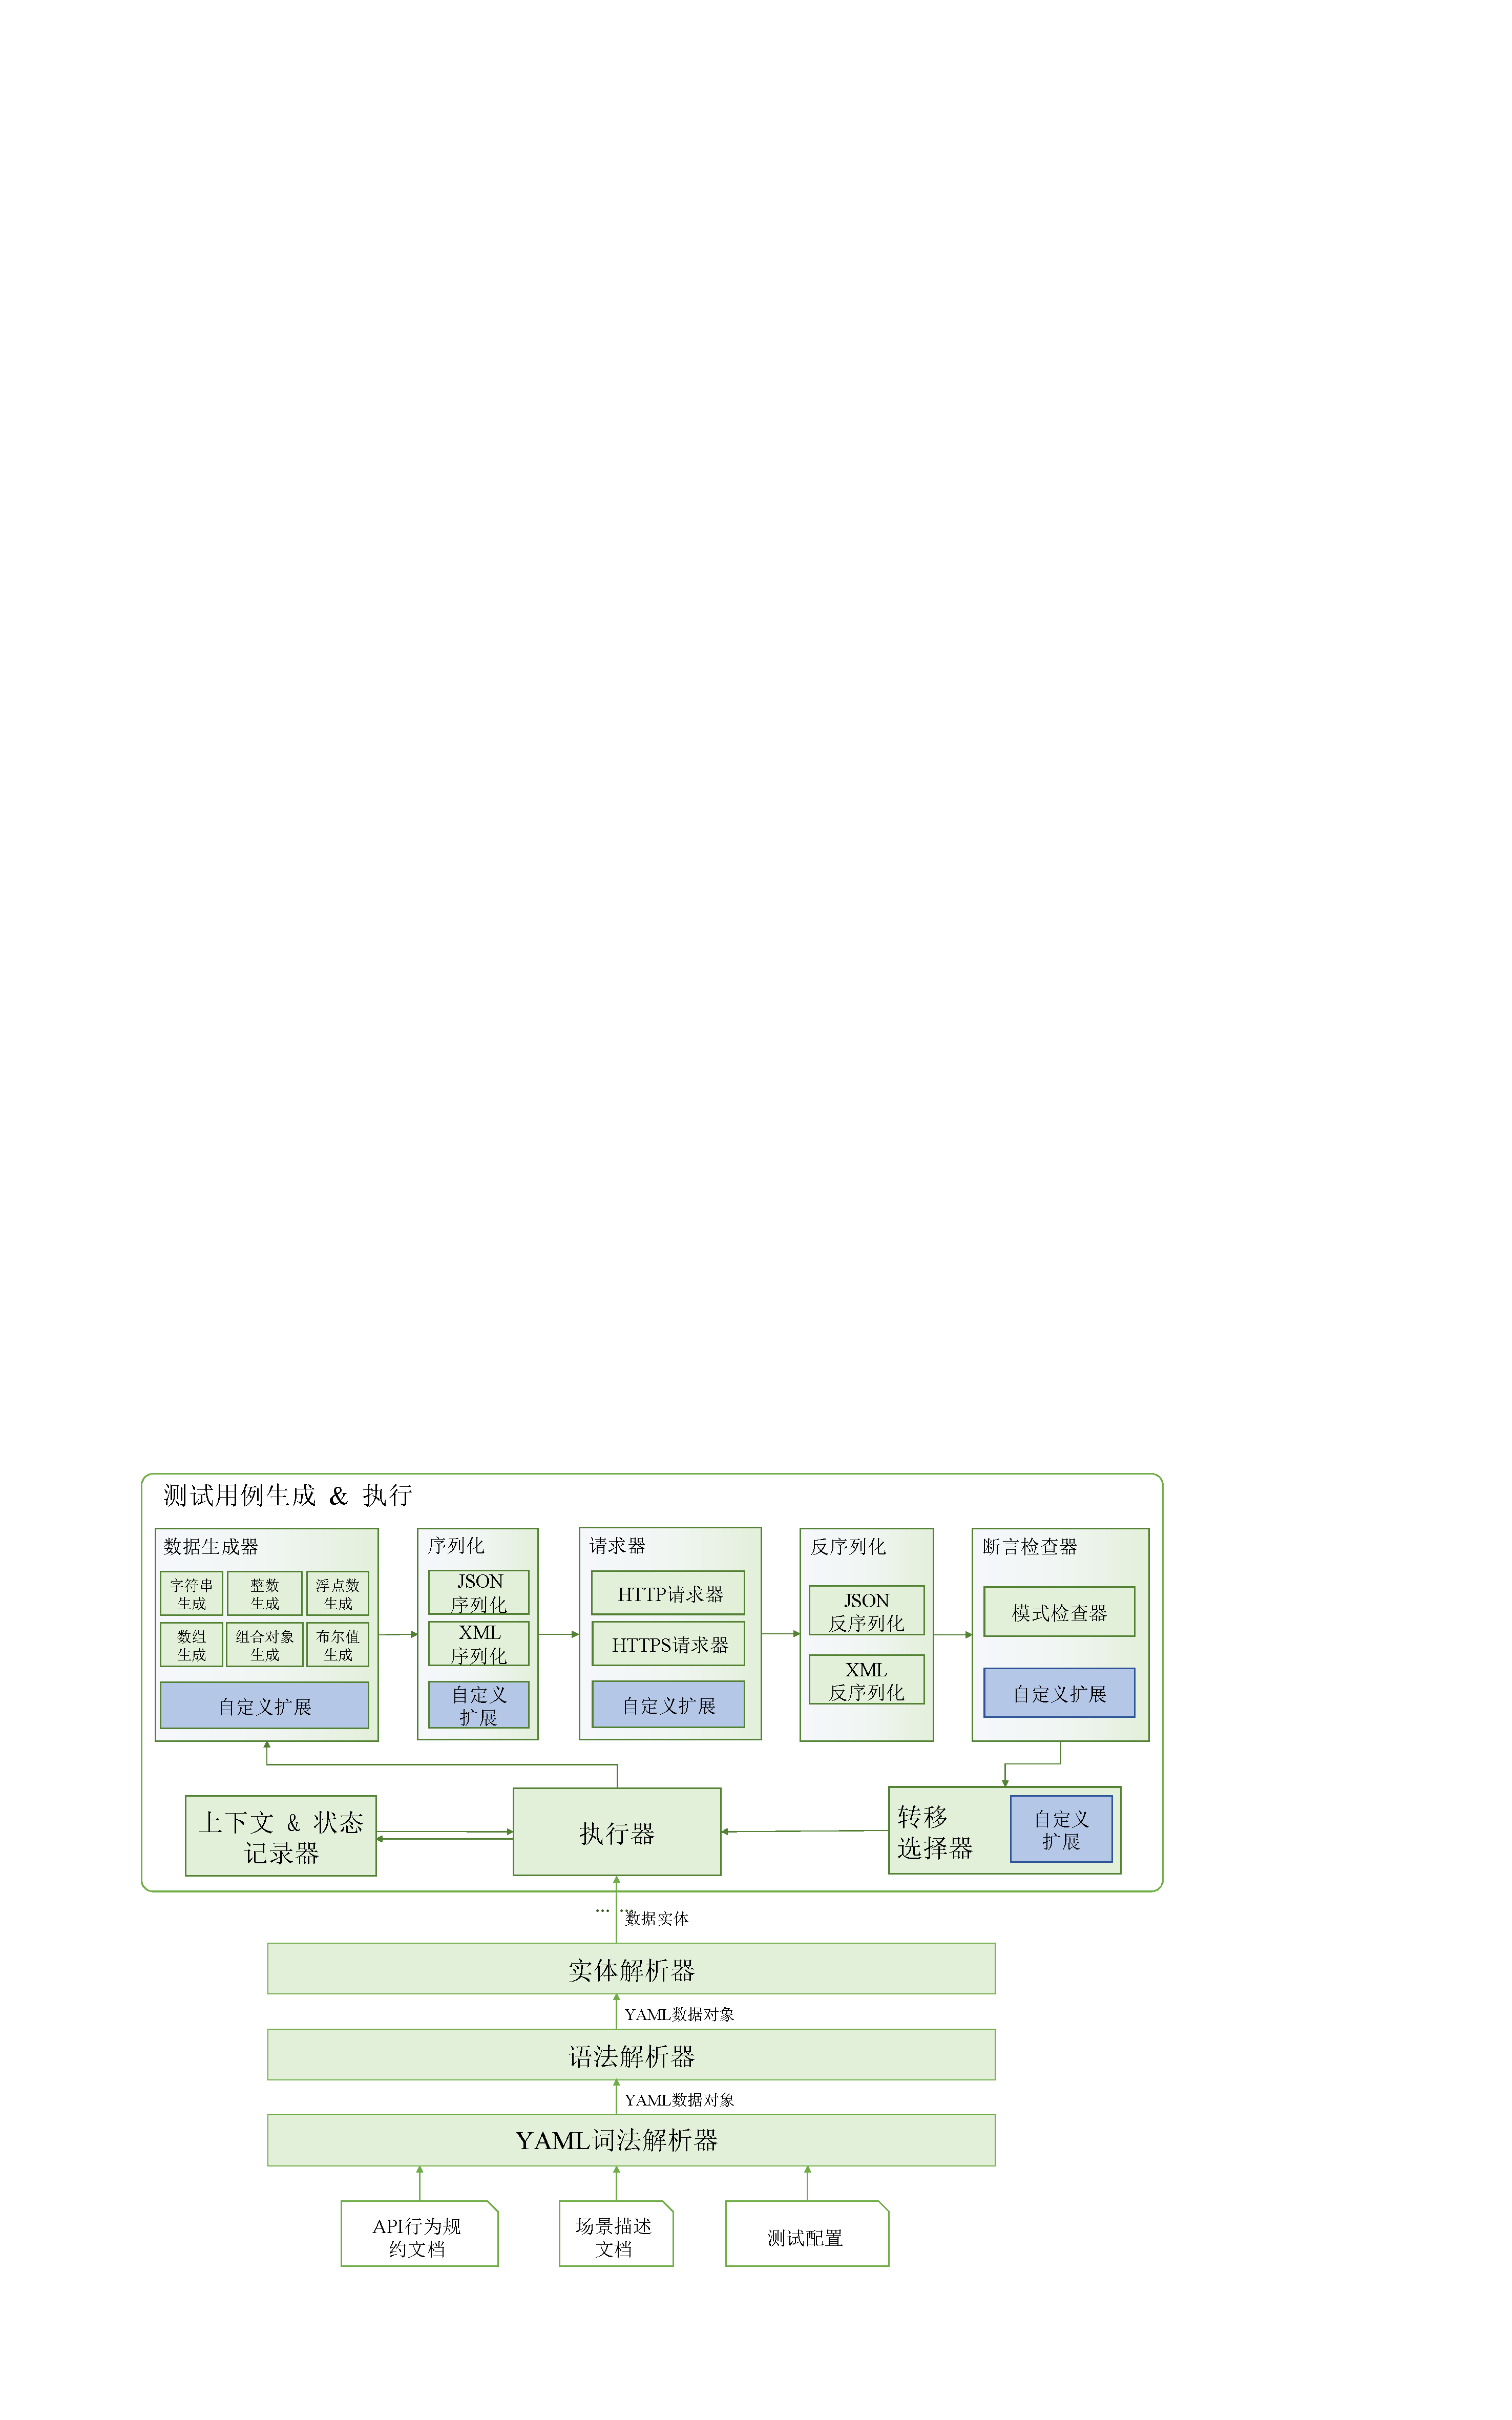
\includegraphics[width=300pt]{tool_architecture3.pdf}
	        \caption{Lapis工具整体架构. 工具的输入为API行为规约文档, 场景描述文档和测试配置. 输出为测试用例及其执行结果. 执行流从下往上, 从左往右.}
	        \label{fig:lapis_arch}
	    \end{figure}
	    
	    图\ref{fig:lapis_arch}展示了Lapis工具原型的整体架构.
	    
	    工具完全采用Python 3实现. 其依赖于一些Python开源库, 如Requests\footnote{http://docs.python-requests.org}, PyYAML\footnote{https://pyyaml.org}, rstr\footnote{https://pypi.org/project/rstr/2.1.1}, 以及标准库.
	    
	    工具的输入为三个脚本文件 - 使用OpenAPI格式描述的API行为文档, 场景模型文档, 以及测试配置文档. 本工作定义了一套格式规范, 用于表述场景模型. 测试配置文档为可选项, 内容较简单, 对API行为文档进行了少量补充, 并提供定制运行参数的功能. 三个脚本文件均为YAML格式. 它们具有着一定的层次关系: API行为文档提供了API的具体定义, 包括请求和响应的格式定义(即场景模型中状态定义的合法请求集合与合法响应集合)和请求方法, 请求URL, 请求协议等; 场景模型文档利用这些信息, 并将场景模型的状态与对应API定义关联起来, 同时为自动化测试提供具体的场景模型; 测试配置文档则提供为定义提供了补充, 并支持一些可定制选项, 如指定测试用例生成与执行的时间限制等.
	    
	    \label{sec:lapis_impl}
	    工具的输出为包含所有测试用例及其执行结果的Python列表, 列表的各个元素即为各个测试用例, 涵盖测试用例的执行序列, 生成的请求数据, 获得的响应结果, 响应时间及模型覆盖率等.

	    工具采用模块化的设计, 具有良好的可扩展性, 如图\ref{fig:lapis_arch}所示, 多个模块均支持用户自定义:
	    \begin{itemize}
	        \item 在场景模型中, 如\ref{sec:set_define}小节所述, 定义合法输入, 合法响应和转移条件可以采用自定义校验函数(对应断言检查器模块的用户扩展)和自定义生成函数(对应数据生成器模块的用户扩展);
	        \item 在请求器中, 为了支持各种不同的API服务, 除了已实现的HTTP协议API请求器和HTTPS协议API请求器外, 用户可以通过子类化抽象接口类的方法进行扩展, 通过这种方式, 可以对使用签名机制的API发送合法请求;
	        \item 在序列化模块中, 除了默认的JSON格式和XML格式序列化模块外, 用户也可以用子类化的方法, 实现自定义的序列化格式;
	        \item 在转移选择器模块中, 除了直接按转移概率随机选择转移外, 用户也可以实现接口函数并在测试配置文档中引入, 以应用启发式的算法;
	        \item 此外, 在全局测试配置中, 为了更好地与被测系统(SUT)交互, 工具提供了用于被测系统启动, 停止和序列间隔时操作的函数接口, 在测试配置文档中指定实现的函数位置, 即可引入自定义交互函数.
	    \end{itemize}  
	    自定义函数和子类的引入得益于Python的动态反射机制, 但这也要求这些自定义扩展使用Python实现.
	    
	    工具各个模块的功能如下:
	    
	    \begin{itemize}
	        \item YAML词法解析器:\\
	            此模块分析输入的三个脚本文件的格式, 分析其是否为合法YAML文档, 并建立文档树.
	        \item 语法解析器:\\
	            此模块读入数据对象, 检查每个脚本是否包括必需域以及各个域的数据合法性, 比如API行为文档中各个API参数的定义是否合法, 场景模型文档中转移的定义是否合法等.
	        \item 实体解析器:\\
	            此模块从脚本中提取出自动化测试所需信息, 而像API描述(\texttt{description}域)和开发者联系方式域(\texttt{info.contact}域)等无关域被舍去. 提取的信息使用数据实体(Python类实例)存储, 并传给测试执行器.
	        \item 测试执行器:\\
	            测试执行器调度和控制整个测试用例的生成和执行过程. 执行器也负责处理用户自定义扩展抛出的异常, 防止系统崩溃. 用户编程接口(见\ref{sec:program_interface}小节)直接与此模块进行交互.
	        \item 上下文\&状态记录器:\\
	            此模块记录测试的所有有用信息, 最后返回给用户.
	        \item 数据生成器:\\
	            此模块生成请求参数(输入数据).
	        \item 序列化:\\
	            此模块将生成的请求参数序列化/格式化为字符串.
	        \item 请求器:\\
	            此模块发送请求, 并收集响应结果. 负责处理网络交互的细节, 也可以进行自定义扩展使之支持签名机制.
	        \item 反序列化:\\
	            此模块将响应的头和响应体分离, 并根据API行为文档和测试配置文档中的数据格式定义, 从字符串解析为数据实体.
	        \item 断言检查器:\\
	            此模块对响应数据进行检查, 包括模式检查(是否符合定义的模式)和断言检查(是否满足上下文依赖和约束)两个方面.
	        \item 转移选择器:\\
	            此模块随机选择转移边, 确定当前执行序列的下一状态.
	    \end{itemize}

	\section{用户接口}
		\subsection{编程接口}
            \label{sec:program_interface}
            用户可以通过调用编程接口直接使用核心工具Lapis. 编程接口为Python函数的形式, 封装并隐藏了工具实现的具体细节. 普通用户使用\texttt{run()}函数, 即可一行完成测试生成与执行. \texttt{run()}函数的签名如下:
            \begin{flushleft}
                \scriptsize
                \tt
                \begin{lstlisting}[language=python]
def run(api_doc_path, scenario_doc_path, testconf_doc_path=None, num_case=1, verbose=0)
                \end{lstlisting}
            \end{flushleft}
            用户需要提供三个脚本文件的路径(测试配置脚本可选), 生成测试用例的总数, 以及往控制台输出信息的详细级别. 输出如\ref{sec:lapis_impl}小节所述, 为包含所有测试用例及其执行结果的Python列表.
            
		\subsection{web端脚本编辑系统}

            本文的工具与方法使用结构化的脚本文档作为输入, 脚本文档则常常需要手工撰写, 因此, 用户友好的脚本编辑和管理工具不可或缺.
            
            本工作为API行为脚本文档的编辑开发了一个在线web系统, 如图\ref{fig:frontend_screenshot}. 在此系统中, 用户可在线编辑与上传API行为脚本, 并获得解析结果的实时反馈. 如果脚本的内容合法, 前端会将所描述的API以类似于使用手册的形式进行可视化, 并展示于右栏. 为了提升可读性, 各个参数和响应体的定义采用折叠式的设计. 如果脚本的内容不合法, 系统会提示出错原因与位置. 每个注册用户拥有私有脚本文件夹, 后台记录了文件夹内各脚本的历史版本, 脚本也可从本地上传到此文件夹. 此外, 编辑系统还附带大量样例方便用户快送熟悉脚本语法.

            \begin{figure}[!htb]
                \centering
                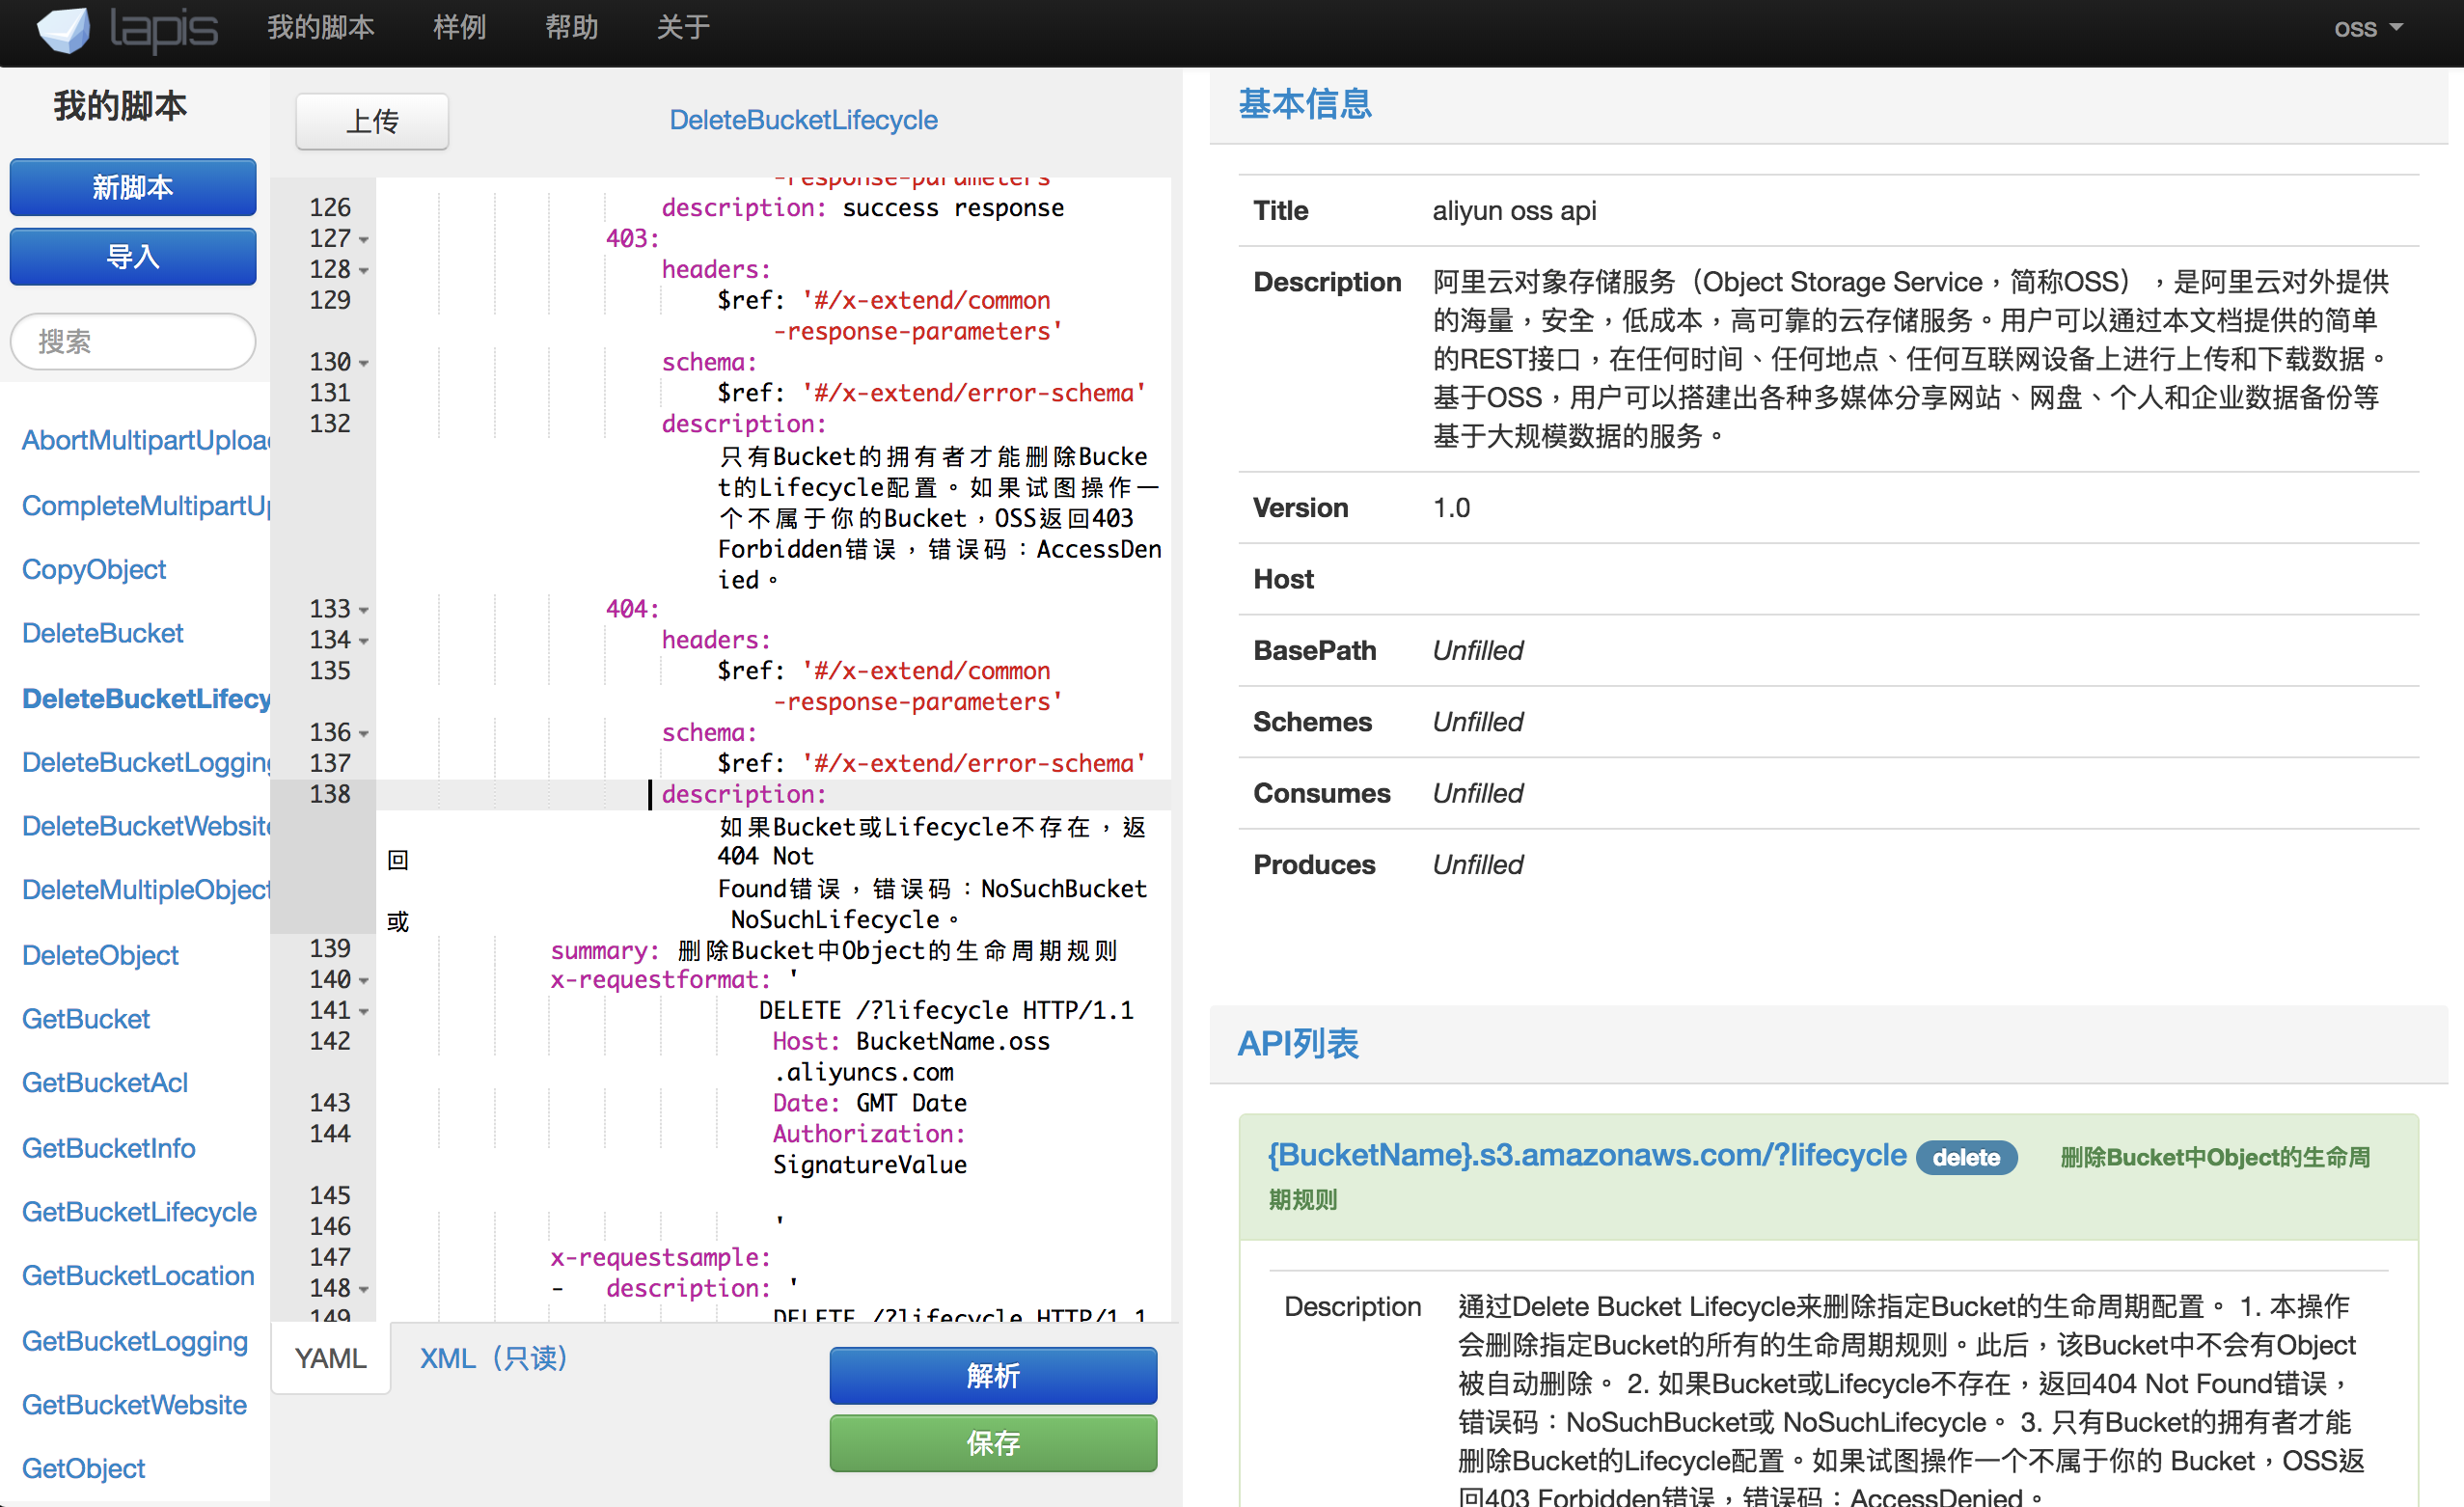
\includegraphics[width=200pt]{frontend_screenshot.png}
                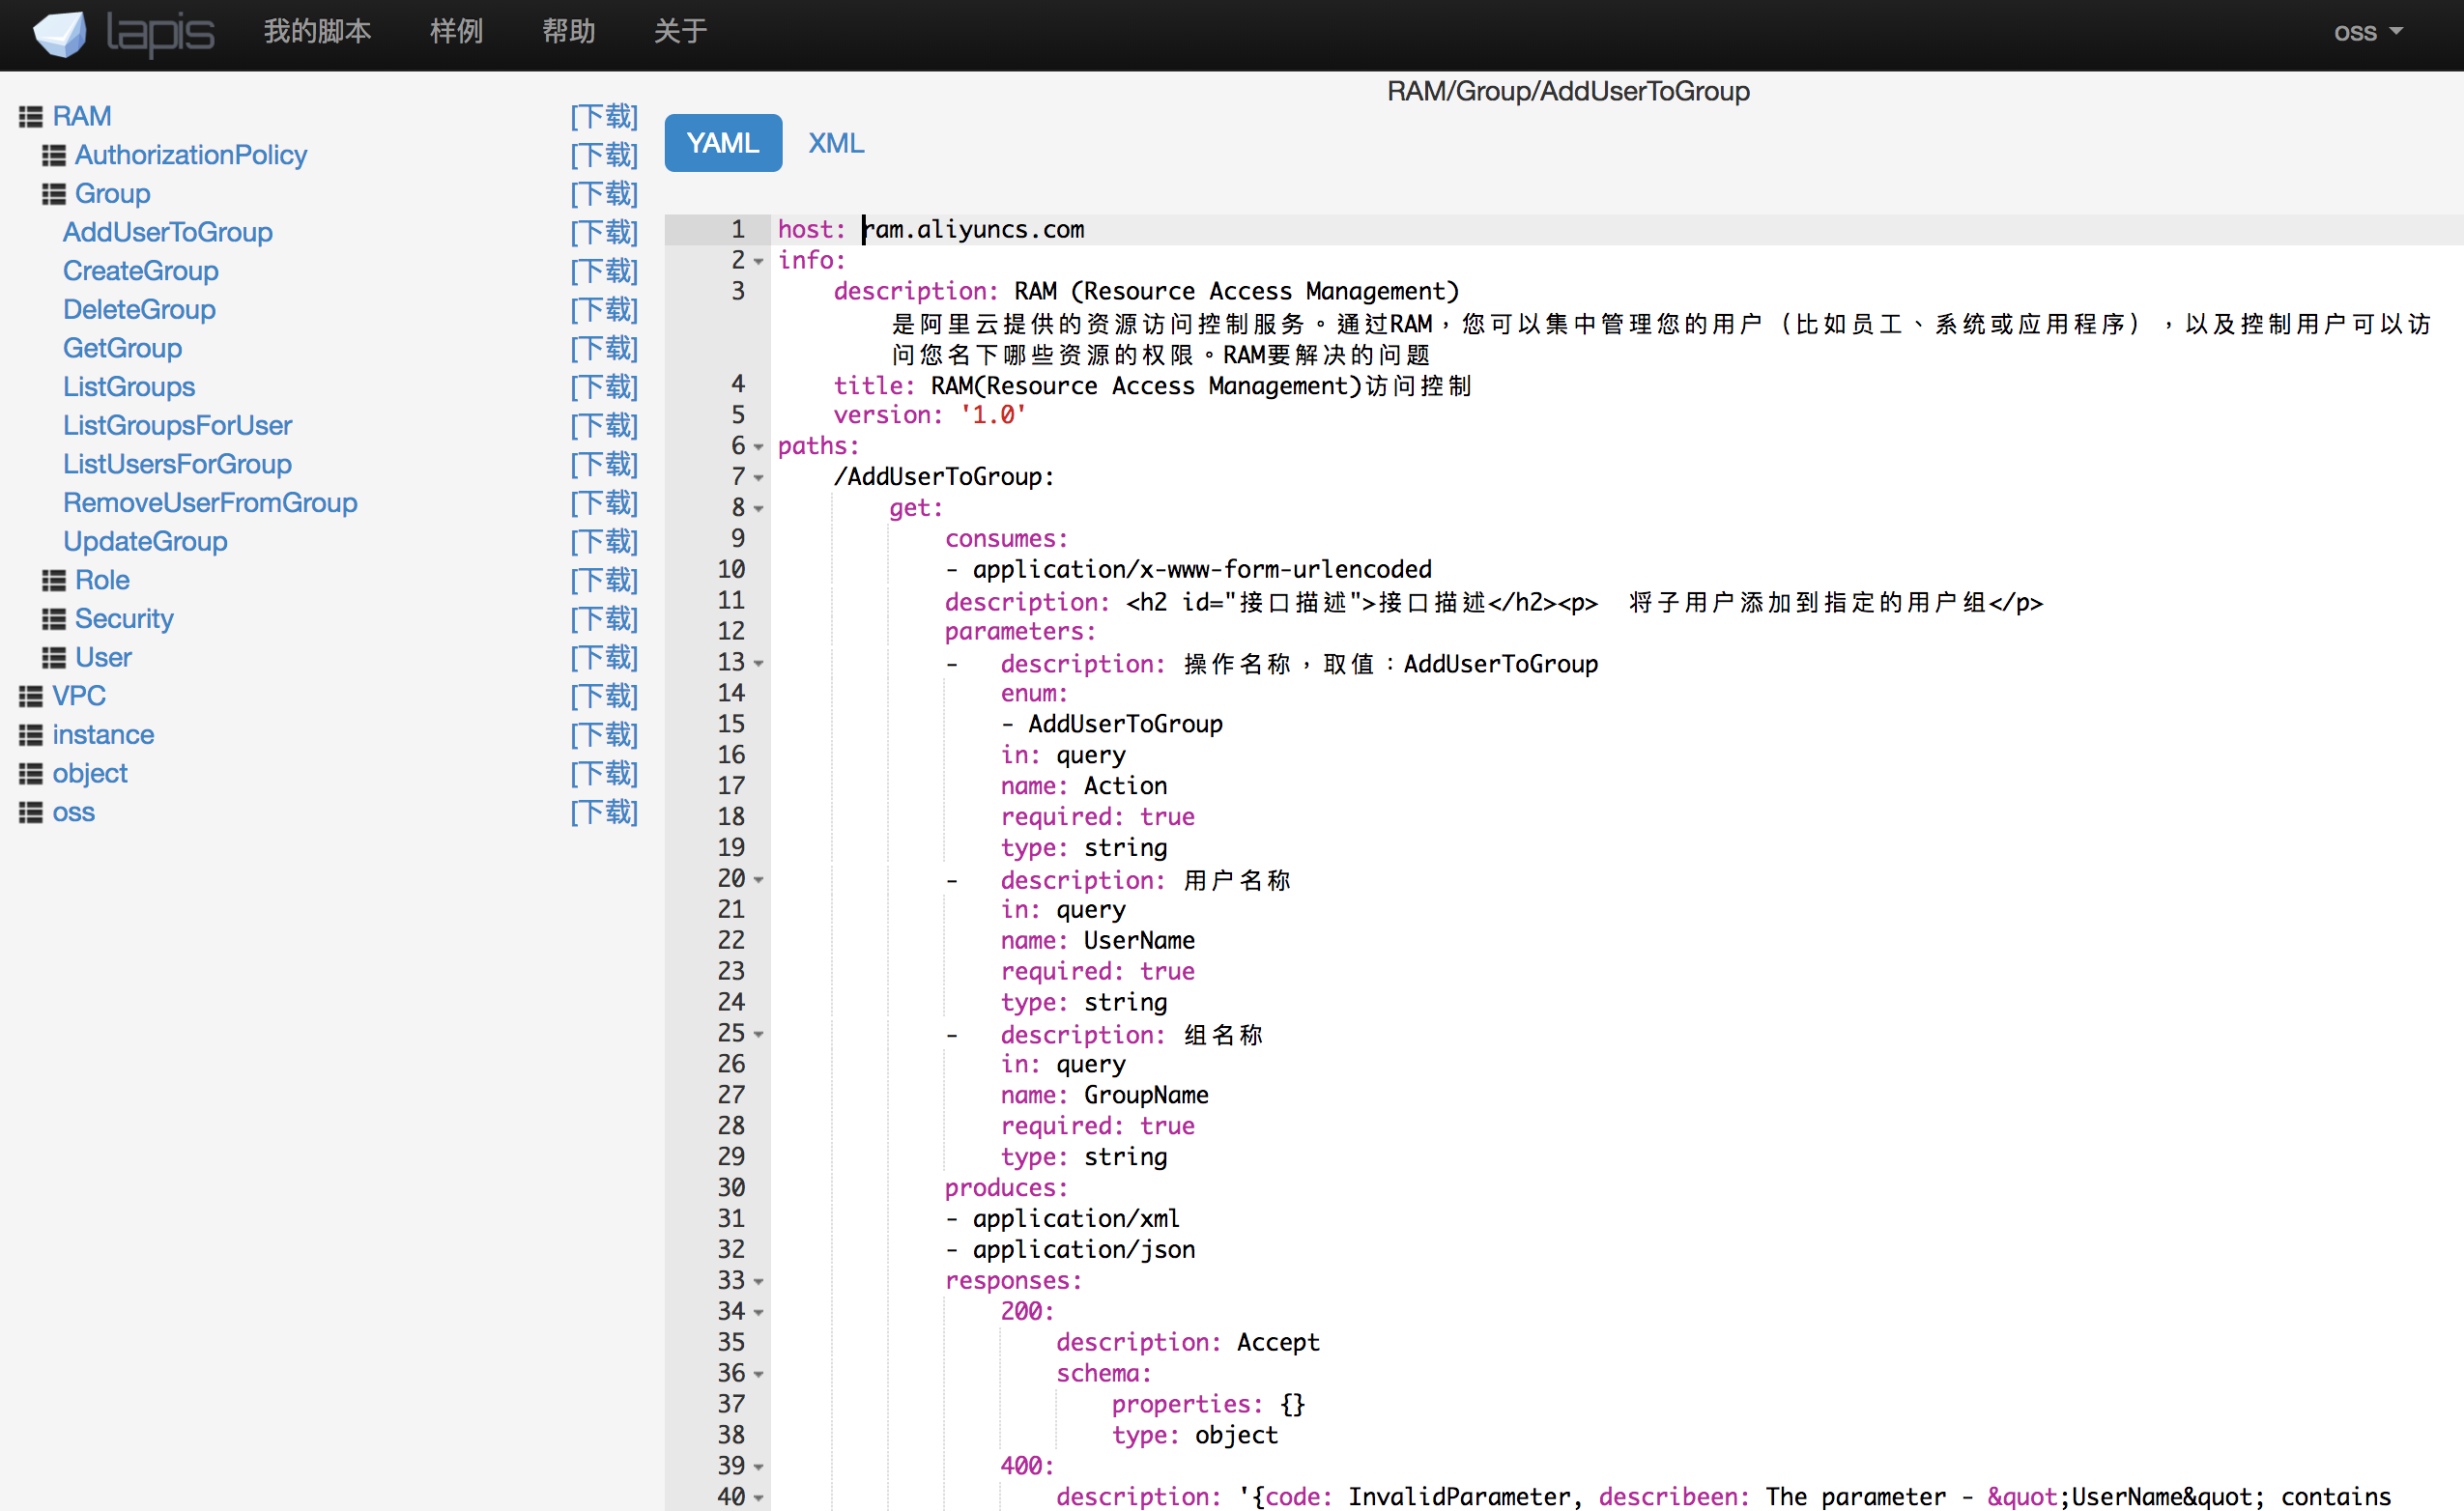
\includegraphics[width=200pt]{frontend_screenshot2.png}
                \caption{Web端脚本编辑系统前端截图. 通过此系统, 用户可以在线进行脚本的编辑与上传, 编辑时, 系统对API脚本进行实时解析, 以类似于API使用手册的形式展示脚本内容.}
                \label{fig:frontend_screenshot}
            \end{figure}
            
            此web编辑系统的后端采用Python语言和Django框架, 前端采用JQuery和Bootstrap库. 直接依托文件系统实现了用户和脚本托管功能, 没有数据库依赖, 十分轻量, 适合部署作为企业测试部门内部服务或单机使用.
        
            此外, 场景模型基于自动机模型, 故场景脚本不适于采用直接撰写的形式, 而适于用有向图表示, 并在图形化界面中拖拽生成\cite{junyiw17}. 开发创建场景模型的图形化界面将明显提高场景脚本的生成效率, 是未来可进一步研究的方向.
            
        % extended version
		% \subsection{*桌面端测试管理系统}



\chapter{实验与评估}



\chapter{总结与展望}





%%% 其它部分
\backmatter

%% 本科生要这几个索引,研究生不要。选择性留下。
% 插图索引
\listoffigures
% 表格索引
\listoftables
% 公式索引
\listofequations


%% 参考文献
% 注意:至少需要引用一篇参考文献,否则下面两行可能引起编译错误。
% 如果不需要参考文献,请将下面两行删除或注释掉。
% 数字式引用
\bibliographystyle{thuthesis-numeric}
% 作者-年份式引用
% \bibliographystyle{thuthesis-author-year}
\bibliography{ref/refs,ref/appendix1bib}

%% 致谢
% 如果使用声明扫描页,将可选参数指定为扫描后的 PDF 文件名,例如:
% \begin{acknowledgement}[scan-statement.pdf]
\begin{acknowledgement}[scan-statement.pdf]
值文章付梓, 闻道清华园, 四载年华, 亦行将结束, 如梭光阴不可追.

当感谢之时, 此只语片言, 远不足道, 仅聊记于此, 涌泉为报必来日.

感谢导师白晓颖副教授. 大二以来, 作为余科研之启蒙导师, 其严谨治学, 嘉言懿行, 为余之学术楷模. 其谆谆教诲, 辛勤指导, 令余常感念师德. 其敬业奉献, 焚膏继晷, 励余以奋发图强. 此三载学术生涯, 使我钟情科研, 决心攻读博士学位. 长忆师恩, 谢无尽焉.

感谢赏识鄙人愚才之各名校教授. 诸先生之栽培授鄙人学术之能力, 诸先生之肯定给鄙人学术之信心, 诸先生之慷慨予鄙人学术之机遇.

感谢诸同窗. 能与诸优秀青年才俊相识相知, 诚本人之荣幸. 诸君之智慧博识, 妙语奇思, 开我思维, 予我灵感. 我的大学生涯因诸君而充实多彩. 尤感谢一同专研本课题并贡献良多的季智成、马浩然同学.

感谢清华大学, 自强不息, 厚德载物之校训, 余将终生谨记于心, 亲力践行. 愿来日为校争光.

衷心感谢自己. 感谢自己不离不弃, 自强不息的四年付出, 感恩成长, 感恩成熟.

最应感恩之人, 必为父母. 感恩双亲养育之恩, 感谢你们带我来到这精彩的世界.

本研究得到国家重点研发计划(项目编号: 2016YFB1000504)的资助, 在此深表感谢.

\end{acknowledgement}


%% 附录
\begin{appendix}

	\chapter{书面翻译}

\title{RESTful API自动化测试用例生成}

\author{Andrea Arcuri\\挪威, 奥斯陆, Westerdals Oslo ACT\\与\ 卢森堡, 卢森堡大学, SnT\\ arcand@westerdals.no}

\begin{cabstract}
当今, web服务在企业级应用的开发中扮演着重要角色. 很多此类应用均采用面向服务的架构(SOA)开发, 微服务是其中最流行的种类之一. 一个RESTful的web服务使用网络上的HTTP协议, 以API的形式提供数据, 也可能与数据库和其他web服务进行交互. RESTful API的输入与输出是对远程服务器的HTTP请求和响应, 因此, RESTful API的测试面临着挑战. 由于被测API是远程服务, 它的代码不可获得, 因此许多相关文献均采用黑盒测试的方法. 在本论文中, 我们站在开发者的角度思考测试 - 所有代码均是可获得的. 因而, 我们提出了一种全自动的白盒测试方法, 其中, 测试用例使用一种进化算法自动生成. 测试用例根据代码覆盖率和故障检测的相关指标给予奖励. 我们在名叫“EvoMaster”的开源工具中实现了这一方法. 在两个开源且有价值的RESTful服务和一个工业界的RESTful服务上的实验结果说明, 我们的新方法可以自动发现这些应用中的38个真实故障. 然而, 代码覆盖率仍比这些服务中已存在的手写测试套件要低. 进而, 我们对如何进一步改进这类方法的可能研究方向进行了讨论.
\end{cabstract}

\ckeywords{REST, SBSE, SBST, SOA, 微服务, Web服务, 测试生成}


\section{引言}
在企业体系中, 面向服务的架构(SOA), 特别是微服务架构\cite{newman2015building}, 已成为常规实践. SOA服务的市场规模在2013年已经达到了57亿美元, 这个市场的巨头有IBM, 微软, 甲骨文和SAP等公司. 预计至2020年\footnote{http://www.radiantinsights.com/research/services-oriented-architecture-soa}, 市场规模将达160亿美元. 目前, REST\cite{fielding2000architectural}是在企业体系中开发web服务的最常用方式. 

不仅在许多企业体系内部, 在互联网上,也有许多RESTful web服务. 如ProgrammableWeb\footnote{https://www.programmableweb.com/api-research}, 在互联网平台上, 目前已有超过16,000项Web API. 在Java生态系统中, 根据对1,700名工程师的调查\footnote{http://www.infoworld.com/article/3153148/java/oracle-survey-java-ee-
users-want-rest-http2.html}, 对REST的更好支持(与HTTP/2支持一同)是在下一代Java企业版(当时为JEE8)中最期待的特性. 根据那项调查, 这是因为“当前Java中的云开发实践在很大程度上基于REST和异步”. 

测试web服务, 尤其是RESTful的web服务, 有许多挑战\cite{canfora2006service}\cite{bozkurt2013testing}. 特别针对服务组合的复杂性, 和黑盒测试外部服务, 业已提出了各种技术. 当前的许多工作着重于处理SOAP的web服务. SOAP是一种基于XML的有完善定义的协议. 然而, 许多企业现已切换到REST服务, REST服务通常使用JSON(JavaScript对象表示法)作为消息本体的数据格式. 此外, 对于web服务的白盒测试, 由于需获得这些服务的源代码, 因此相关研究工作还较少. 

在本论文中, 我们提出了一种可以自动化生成RESTful web服务的集成测试的新方法. 我们的方法有两个主要目标: 最大化代码覆盖率(如语句覆盖率), 和使用HTTP返回状态码作为自动化测试参照物来检测故障. 我们的目标是在独立环境中测试RESTful服务, 这是工程师在开发服务时直接进行的一种典型测试类型. 为了生成测试, 我们使用了一种进化算法, 具体来说, 是使用整测试套件方法的遗传算法\cite{fraser2013whole}. 

我们实现了一个名叫EvoMaster的工具原型, 并在三个不同的RESTful web服务上进行了实验. 其中两个服务是开源的, 第三个则由我们的一个工业界伙伴提供. 这些系统的代码行数从两千到一万行不等. 实验结果显示, 新方法可以在这些系统上发现38个真正的故障. 但是, 与已有的手写测试用例相比, 代码覆盖率还相对较低. 这主要是因为字符串约束和与数据库, 外部web服务的交互的存在. 要解决这些问题并进一步改进表现, 则还需要进一步的研究.

特别地, 这篇论文提供了以下的研究与工程贡献: 

\begin{itemize}
\item 针对RESTful的web服务, 我们设计了一个可生成有效测试用例的新技术.
\item 我们提出了一种自动化分析, 导出和利用web服务的白盒信息, 来改进测试数据生成的方法.
\item 我们展示了其在真实软件上的实证研究, 研究表明, 尽管工具还在早期的原型阶段, 它已经能自动发现这些RESTful web服务中的38项真正的故障.
\item 为了使我们的结果, 工具对比, 和算法实现具有可重复性, 我们遵守开源LGPL协议发布了工具原型, 并发布于公共托管仓库GitHub\footnote{https://github.com/arcuri82/EvoMaster}上.
\end{itemize}
  
\section{背景}
  \subsection{HTTP}
      超文本传输协议(HTTP)是网络通信的一种应用协议, 也是万维网(World Wide Web)上通信的主要协议. HTTP协议由一系列征求意见稿(RFC)文档定义, 这些征求意见稿由互联网工程任务组(IETF)和万维网联盟(W3C)维护, 比如RFC7230\footnote{https://tools.ietf.org/html/rfc7230}和RFC7231\footnote{https://tools.ietf.org/html/rfc7231}. 
        
        一个HTTP消息通常在TCP之上传输, 由四个主要部分组成: 
        \begin{itemize}
          \item \textit{原语/方法}: 要进行的操作类型, 如获取某特定网页. 
          
            \item \textit{资源路径}: 指定HTTP操作所应用的资源的标识符, 如要获取的HTML文档的路径. 
            
            \item \textit{头}: 额外的元信息, 由一个键值对的列表表示. 如, “accept”头是一种元信息, 它用来指定资源返回时的格式(如HTML, XML或JSON)(资源可以有多种可用的格式). 
            
            \item \textit{体}: 消息的载荷, 如作为“get”请求的响应而返回的HTML文本. 
        \end{itemize}
        
        HTTP协议在公开的资源上允许以下操作(即原语/方法): 
        \begin{itemize}
          \item \textit{GET}: 指定的资源应该在响应体中返回. 
            \item \textit{HEAD}: 类似GET, 不过被请求资源的响应体不应该被返回. 当用户只需要检查资源是否存在时, 或者用户只需要获取响应头时, 这一操作很有用. 
            \item \textit{POST}: 向服务器发送数据, 如web表格的文本值. 通常, 当需要指定新资源在服务器上创建时, 会使用这一方法. 
            \item \textit{DELETE}: 删除指定资源. 
            \item \textit{PUT}: 将指定资源用新资源替代, 新资源在请求体中指定. 
            \item \textit{PATCH}: 对指定资源做局部更新. 与PUT方法相比, PUT方法则是将已有资源用新资源完全替换. 
            \item \textit{TRACE}: 回传收到的请求. 当我们想确定HTTP请求是否有被客户和服务器之间的中间者(如代理)篡改时, 这个方法很有用. 
            \item \textit{OPTIONS}: 列出给定资源的所有可用HTTP方法. 举个例子, 某个HTML文件可以使用GET方法, 但是不能使用DELETE方法. 
            \item \textit{CONNECT}: 通过HTTP代理建立隧道连接, 通常在加密通信中使用. 
        \end{itemize}
        
        当客户发送一个HTTP请求后, 服务器会送回一个有头和可选的请求体载荷的HTTP响应. 此外, 响应还会包含一个三位数字的状态码. 状态码有五个组/系列, 组别靠第一位数字区分: 
        \begin{itemize}
          \item \textit{1xx}: 用于临时响应, 如确认协议切换(101), 或对于某个之前的只获取响应头的条件请求, 应继续发送响应体(100). 
            \item \textit{2xx}: 响应被成功处理时返回(200). 具体地, 作为POST命令的结果, 服务器还可以进一步表明一个资源被创建了(201); 或作为DELETE命令的结果, 表明不需期望有响应体(204).
            \item \textit{3xx}: 此组状态码被用于重定向, 如告诉用户被请求的资源现在在其他位置可用. 重定向可以是临时的(307)或永久的(301). 
            \item \textit{4xx}: 用于指定用户请求无效(400). 一种典型情景是被请求资源不存在(404), 或试图在未被认证的情况下(401)或未被授权的情况下(403)获取被保护的资源. 
            \item \textit{5xx}: 当服务器不能提供有效响应时返回(500). 一种典型情景是业务逻辑代码有故障且在请求处理时抛出异常, 然后异常被应用服务器捕获(故当异常被抛出时, 整个服务器不会崩溃). 然而, 在用到的外部服务(如数据库)没有正确响应时也会返回这类响应吗. 比如当数据库的硬盘损坏时, 尽管服务器不能再使用数据库, 它仍可以返回500作为HTTP响应.
        \end{itemize}
    
      HTTP协议是\textit{无状态}的: 因为HTTP协议不存储任何之前的信息, 每个进入的请求都需要提供处理所需的所有信息. 为了在用户进行的一些相关HTTP请求间维护状态(如购物车), 需要使用\textit{cookies}: \textit{cookies}是服务器创建的用来识别指定用户的有唯一id的HTTP头, 用户需要在他的所有HTTP请求中包含这个HTTP头.
    
    \subsection{REST}
      多年以来, 编写web服务的主要方式是使用SOAP(简单对象访问协议), 这是一个使用XML包装信息的通信协议. 然而, 近年来, 在开发web服务时, 工业界有明显的向REST(表现层状态转移)过渡的趋势. 许多巨头已在使用REST, 如Google\footnote{https://developers.google.com/drive/v2/reference/}, Amazon\footnote{ http://docs.aws.amazon.com/AmazonS3/latest/API/Welcome.html}, Twitter\footnote{https://dev.twitter.com/rest/public}, Reddit\footnote{https://www.reddit.com/dev/api/}, LinkedIn\footnote{https://developer.linkedin.com/docs/rest-api}等等. 

    REST的概念首先由一篇有很大影响力(目前引用量近6000)的2000年的博士论文\cite{fielding2000architectural}引入. REST不是一个协议(如SOAP那样), 而是一系列在HTTP上设计web服务的架构上的指南. 这种客户端 - 服务器应用需要满足一些约束, 才能被认为是RESTful的, 比如无状态; 资源需被明确指明是否可缓存; 资源需能用URI指定; 由客户端发送的资源表示(JSON或XML)需与资源的实际格式(如关系型数据库的一行)保持独立; 资源需通过合适的HTTP方法管理与组织, 比如某个资源应该由DELETE请求来删除而不是POST请求; 等等.
        
        让我们考虑一个RESTful web服务的例子, 它让我们操作一个产品名录. 这些是可能的操作: 
        \begin{itemize}
          \item \textit{GET /products} (返回所有可用产品)
            \item \textit{GET /products?k=v} (返回由自定义参数过滤的可用产品)
            \item \textit{POST /products} (创建一个新产品)
            \item \textit{GET /products/\{id\}} (返回指定id的产品)
            \item \textit{GET /products/\{id\}/price} (返回指定id产品的价格)
            \item \textit{DELETE /products/\{id\}} (删除指定id的产品)
        \end{itemize}
      注意这些URI并没有指定返回的表示格式. 一个服务器可以用不同的格式提供相同的资源, 如XML或JSON, 并且这个格式应该在请求头中指定. 
        
        REST的另一个特性是所谓的HATEOAS(超媒体即是应用状态引擎), 即每个资源表示也应该提供往其它资源的链接(与网页的链接类似). 举个例子, 当请求\textit{GET /products}时, 不仅仅是所有产品列表应被返回, 还应有到其它可用请求方法的链接. 理想情形下, 给出API的一个主入口, 整个这个API应该能通过这些链接完全发掘到. 然而, HATEOS在实践中很少使用\cite{rodriguez2016rest}, 这主要是因为缺乏定义链接格式的合适规范(如JSON或XML模式), 并且这会给客户端带来额外的负担. 
        
        注意: REST不是协议, 而只是架构指南的集合\cite{fielding2000architectural}, 名词”REST“十分常见, 但在实践中常被误用. 虽然许多HTTP上的Web API严格上讲并不能被认为是完全REST的\cite{rodriguez2016rest}\cite{fielding2000architectural}, 但它们使用REST的冠名与宣传. 虽然在本论文中我们使用术语REST, 但提出的新技术可以用于任何通过HTTP端点访问, 并且载荷数据用类似JSON或XML的语言描述的web API. 
    
    \subsection{基于搜索的软件测试}
    由于软件可以十分复杂, 测试数据生成是一项复杂的任务. 而且, 很多开发者都感觉编写测试用例枯燥乏味. 因此, 有许多相关研究旨在实现自动化生成高质量测试用例. 其中一个最简单的方法是随机生成测试用例\cite{arcuri2012random}. 虽然在一些场景中随机可能是很有效的, 但这可能仅仅只能覆盖被测软件的一小部分. 比如, 由于一个随机生成的字符串几乎不可能构成一个有效且符合格式的HTTP消息, 在RESTful API上使用裸随机测试策略是没有多少意义的. 
        
        在多年来提出的许多不同测试技术中, 基于搜索的软件工程在解决许多软件工程问题中都格外有效\cite{harman2012search}, 尤其是在软件测试中\cite{ali2010systematic}, 如单元测试生成的高级工具EvoSuite\footnote{ https://github.com/EvoSuite/evosuite}\cite{fraser2011evosuite}\cite{fraser2014large}. 软件测试可以被建模为一个优化问题, 目标是最大化生成的测试套件的代码覆盖率和故障检测率. 进而, 只要对于给定的测试问题定义了适应度函数, 便可使用搜索算法来探索可能解的空间(在此上下文中为测试用例). 
        
        有许多种类的搜索算法, 其中遗传算法(GA)可能是最为著名的. 在遗传算法中, 使用个体的集合来进行多代进化. 根据适应度值, 首先选择一些个体繁衍, 然后, 在采样新后代时, 使用杂交(混合来自父母双方的基因)和突变(小尺度变化). 当最优个体出现时, 或者搜索过程用尽了分配的时间时, 进化结束.

\section{相关工作}
  Candora和Di Penta讨论了SOA(面向服务架构)测试的趋势和挑战\cite{canfora2006testing}. 之后, 他们发表了一篇更详细的综述\cite{canfora2006service}. SOA的测试有许多不同的类型(单元测试, 集成测试, 回归测试, 鲁棒性测试等等), 参与者的角色也很多样, 有服务开发方, 服务提供方, 服务集成方, 第三方验证方等等. Bertolino等人\cite{bertolino2012trends}也讨论了SOA验证的趋势和挑战. 
    
    在这之后, Bozkurt等人\cite{bozkurt2013testing}也发表了关于SOA测试的综述, 在其中分析了177篇论文. 这篇综述的一项有趣结果是, 虽然近几年来关于SOA测试的论文数量一直在增加, 但只有11\%的论文提供了在实际系统上的实证实验. 71\%的论文完全没有提供任何实验结果, 甚至是试验系统上的实验也没有提供. 
    
    在这一领域内的许多工作集中在使用WSDL(Web服务描述语言)描述的SOAP web服务的黑盒测试上. 正如\cite{xu2005testing}\cite{bai2005wsdl}\cite{martin2006automated}\cite{ma2008wsdl}\cite{bartolini2009ws}\cite{li2016generating}, 人们提出了许多不同的策略. 如果这些服务也提供了语义模型(如使用OWL-S格式), 那么我们可以利用它来生成更“实际”的测试数据\cite{bozkurt2011automatically}. 当在SOA中的服务组件采用BPEL(Web服务业务流程执行语言)来描述时, 我们可以使用许多不同的技术来为这些组件生成测试\cite{wotawa2013fifty}\cite{jehan2014soa}. 
    
    黑盒测试有它的优势, 但也有它的限制. 使用覆盖率指标可以提高测试生成的质量, 但是, web服务常常位于远程, 因而无法获取到源代码. 对于测试, Bartolini等人\cite{bartolini2011bringing}提出了一种将代码覆盖率反馈作为服务提供的方法, 该反馈不会暴露被测web服务的内部细节. 然而, 代码覆盖率探针的插桩必须手动完成. Ye和Jacobsen\cite{ye2013whitening}也提出了一种相似的方法. 在本论文中, 我们提出的方法也将代码覆盖率作为服务提供, 但却是全自动的(基于即时字节码操作). 
    
    对于RESTful web服务, Chakrabarti和Kumar\cite{chakrabarti2009test}提供了一套测试框架, 该框架“根据穷举所有请求参数值的有效组合来自动生成测试用例”.  Seijas等人\cite{lamela2013towards}提出了一种以理想化的, 基于属性的测试模型为基础, 进行RESTful API测试生成的技术. Chakrabarti和Rodriquez\cite{chakrabarti2010connectedness}定义了一种形式化RESTful web服务的“连通性”, 并根据此模型生成测试的技术. 有形式化模型时, 一些技术就也可以使用了, 比如\cite{pinheiro2013model}和\cite{fertig2015model}中的技术. 我们的技术与以上技术都有着显著不同, 这体现在我们的技术不需要任何形式化模型的存在, 并且可以自动利用白盒信息, 且使用进化算法来指导生成有效测试.
    
    关于进化算法在web服务测试中的应用, Di Penta等人\cite{di2007search}为测试服务水平协议(SLA)提出了一种方法. 给定一个有着形式化协议的API, 比如“服务提供方保证服务购买者获得少于30 ms的响应时间与不低于300 dpi的解析度”, 便可以使用进化算法来生成不满足协议的测试用例. 适应度函数可以基于测试用例与违反被测协议之间的距离, 此函数的值可以在执行后求得. 

\section{方法}

  在这篇论文中, 我们提出了一种对RESTful API的web服务自动化生成测试用例的新方法. 我们考虑在孤立环境中测试RESTful服务, 而不是作为两个或更多一起运行的服务的一部分(如在微服务架构中)来测试. 对应的应用场景是: 这些RESTful服务的开发者可以直接使用我们的方法来自动生成测试用例. 因此, 我们假设这些服务的源代码是可获得的. 目标则是生成有高代码覆盖率, 并且能检测出当前服务实现中的故障的测试用例. 因此, 我们需要定义什么是测试用例, 什么可以被用来作为自动化测试的参照(需要检测故障行为), 以及搜索算法如何被用来生成这类测试. 
    
    \subsection{测试用例}
    在我们的语义中, 一个测试用例是对一个RESTful服务的一个或多个HTTP请求. 因此, 测试数据可被视为一个代表HTTP请求的字符串. 然而, 除了给定的HTTP请求结构(如头和资源路径里的参数), 测试数据还可以复杂得多. 比如请求体部分的内容就可以是任何格式. 因为目前JSON是RESTful API通信的主要格式, 在这篇论文中我们只关注这一格式. 若要使之处理其他使用频率较小的格式, 比如XML, 则只需要一些工程上的实现即可. 
    
    在能够发送HTTP请求之前, 首先我们需要知道哪些API方法是可用的. 相比于有完善定义的SOAP协议, REST并没有一个用来定义可用API的标准. 但是, 有一个非常流行的REST文档化工具叫Swagger\footnote{http://swagger.io}, 它目前支持多于25种不同的程序语言. 另一个不太知名的工具叫RAML\footnote{http://raml.org}. 当一个RESTful API用Swagger配置后, 它将自动提供一个JSON文件作为资源, 这个文件完全定义了在此RESTful服务里, 存在着哪些API. 因此, 在测试这个RESTful服务之前, 第一步就是提取出Swagger的JSON定义. 
    
    图\ref{fig1}展示了我们将在实证研究中使用的一个系统的Swagger定义的片段. 这个JSON文件总计超过2000行代码. 如图所示, 对同一个资源, 有两个HTTP操作的定义(GET和PUT). 为了在这个资源上执行GET操作, 需要两个值: 作为资源路径一部分的数字值“id”, 和一个可选的查询参数“attrs”. 譬如, 给出模板“\textit{/v1/activities/\{id\}}”, 我们可以对“\textit{/v1/activities/5?attrs=x}”发出请求. 
    
    PUT操作也需要“id”的值, 但是不需要可选参数“attrs”. 此外, 在它的HTTP请求体里, 可以有一个用JSON表达的资源用于替换, 此处名为“ActivityProperties”. 图\ref{fig2}展示了这个对象的定义. 这个对象有许多不同类型的域, 如数值(如“id”), 字符串(如“name”), 日期(如“date\_published”), 数组(如“tags”)和一些其他对象(如“author”). 为这种PUT操作编写测试用例时, 不仅仅需要确定路径中的“id”, 还需要这种“ActivityProperties”对象的实例, 并且需要将之整理为一个JSON字符串来加入到HTTP请求的请求体中. 
    
    \begin{figure}
      {
      \tt
        \scriptsize
      \begin{lstlisting}[language=C++]
"/v1/activities/{id}": { 
  "get": {
    "tags": [ 
      "activities"
    ],
    "summary": "Read a specific activity", 
    "description": "",
    "operationId": "get",
    "produces": [
      "application/json" 
    ],
    "parameters": [ 
      {
        "name": "id", 
        "in": "path", 
        "required": true, 
        "type": "integer", 
        "format": "int64"
      }, 
      {
        "name": "attrs",
        "in": "query",
        "description": "The attributes to include in the response. Comma-separated list.", 
        "required": false,
        "type": "string" 
      }
    ], 
    "responses": {
      "default": {
        "description": "successful operation"
      } 
    }
  }, 
  "put": {
    "tags": [ 
      "activities"
    ],
    "summary": "Update an activity with new information.
Activity properties not specified in the request will be cleared.", 
    "description": "", 
    "operationId": "update", 
    "produces": [
      "application/json" 
    ],
    "parameters": [ 
      {
        "name": "id", 
        "in": "path", 
        "required": true, 
        "type": "integer", 
        "format": "int64"
      }, 
      {
         "in": "body", 
         "name": "body", 
         "required": false, 
         "schema": {
          "$ref": "#/definitions/ActivityProperties"
        }
      }
    ],
    "responses": {
      "200": {
        "description": "successful operation",
        "schema": {
          "$ref": "#/definitions/Activity"
        }
      }
    }
  }
        \end{lstlisting}
        }
      \caption{对\textit{/v1/activities/\{id\}}资源的两个操作(GET和PUT)的Swagger JSON定义}
        \label{fig1}
    \end{figure}
    
    \begin{figure}
      {
        \tt
        \scriptsize
      \begin{lstlisting}[language=C++]
"ActivityProperties": { 
  "type": "object", 
  "properties": {
    "id": {
      "type": "integer", "format": "int64"},
    "name": {
      "type": "string",
      "minLength": 0, "maxLength": 100 },
    "date_published": { 
      "type": "string", "format": "date-time"},
    "date_created": { 
      "type": "string", "format": "date-time"},
    "date_updated": { 
      "type": "string", "format": "date-time"},
    "description_material": {
      "type": "string",
      "minLength": 0, "maxLength": 20000},
    "description_introduction": {
      "type": "string",
      "minLength": 0, "maxLength": 20000},
    "description_prepare": {
      "type": "string",
      "minLength": 0, "maxLength": 20000},
    "description_main": {
      "type": "string",
      "minLength": 0, "maxLength": 20000},
    "description_safety": {
      "type": "string",
      "minLength": 0, "maxLength": 20000},
    "description_notes": {
      "type": "string",
      "minLength": 0, "maxLength": 20000},
    "age_min": {
      "type": "integer", "format": "int32",
      "maximum": 100.0},
    "age_max": {
      "type": "integer", "format": "int32",
      "maximum": 100.0},
    "participants_min": {
      "type": "integer", "format": "int32"},
    "participants_max": { 
      "type": "integer", "format": "int32"},
    "time_min": { 
      "type": "integer", "format": "int32"},
    "time_max": { 
      "type": "integer", "format": "int32"},
    "featured": { 
      "type": "boolean", "default": false},
    "source": {
      "type": "string"},
    "tags": {
      "type": "array",
      "xml": {"name": "tag", "wrapped": true}, 
      "items": {"$ref": "#/definitions/Tag"}},
    "media_files": {
      "type": "array",
      "xml": {"name": "mediaFile", "wrapped": true}, 
      "items": {"$ref": "#/definitions/MediaFile"}},
    "author": {"$ref": "#/definitions/User"}, 
    "activity": {"$ref": "#/definitions/Activity"}
  }
}
        \end{lstlisting}
        }
        \caption{一个复杂对象类型的Swagger JSON定义}
        \label{fig2}
    \end{figure}
    
    \subsection{参照}
    当使用白盒方法自动生成测试用例时, 比如努力最大化语句覆盖率时, 使用什么来作为自动\textit{参照}是一个问题\cite{barr2015oracle}. 参照可以被视为一个判断测试用例的结果是否正确的函数. 在手动测试中, 开发者确定对于给定测试用例的期望结果, 并将期望编写成断言以在测试用例里直接检查. 在自动测试生成中, 一次有成百上千的测试用例被产生, 这时候让开发者写断言就不是一种可行的选择了. 
        
  对参照问题并没有简单的解决办法, 不同的方法都有不同程度的成功但也有不同程度的局限\cite{barr2015oracle}. 在系统级别的测试中, 最明显的自动参照是检查当测试执行后整个被测系统是否崩溃(如C程序的段错误). 这种测试用例可以检测出软件故障, 但是不是所有故障都会导致应用的完全崩溃(有可能只是一小部分的故障是这种类型的). 另一种方法是编写形式化的规约(如前置/后置条件)作为自动参照, 但是这些在实际中较少使用. 
        
  在单元测试中, 我们可以查看被测类/方法抛出的异常\cite{fraser20151600}. 然而, 这里的一个主要问题是, 抛出的异常很多时候并不是故障的征兆, 而只是表明违反了未明确的前置条件(如输入为空, 但目标函数并没被要求需在空输入上运行). 
        
  尽管没有自动参照, 在\textit{回归测试}中生成的测试用例仍然是有用的. 举个例子, 如果一个被测函数$foo$接受一个整型数作为输入, 然后返回一个整型数作为计算结果, 那么一个自动生成的测试用例可以在一个断言中捕获到函数的当前行为, 举个例子: 
        
    {
        \tt
        \small
        \begin{lstlisting}[language=java]
int x = 5;
int res = foo(x);
assertEquals(9, res);
    \end{lstlisting}
    }
        
    现在, 测试生成工具可以选择生成一个测试用例, 其中输入值$x = 5$, 但是它不能知道是否应该期望输出为9(这是调用$foo(x)$的实际返回值). 开发者可以阅读测试用例, 然后确定是否9真的是期望的输出. 但是, 即使他不检查这个测试用例, 这个测试用例也会被加入到当前的测试用例集内, 然后作为连续集成过程(如Jenkins\footnote{https://jenkins.io})的一部分, 在每次有新代码变更时执行. 如果一次源代码的修改导致$foo$在输入为5时返回了不等于9的结果, 那么这个测试用例就会失败. 在这个时候, 开发者就有必要检查是否最近的变更导致了此函数出现错误(如果这是一个故障), 或者是否此函数的语义发生了变化.
        
    在RESTful API中, 生成的测试用例还可被用于回归测试. 测试用例在安全领域也十分有用: 比如, 一个引发403(未认证)状态返回的HTTP调用可以探测出权限检查被错误放宽的回归时故障. 状态码还可以被进一步用来作为自动参照. 虽然4xx的状态码不能说明RESTful web服务的故障, 但是5xx可以. 如果被测web服务的环境(如数据库)是正常运行的, 则5xx的状态码通常意味着此服务内的故障. 一个典型例子是异常抛出: 如果在RESTful端点处的业务逻辑抛出了异常, 应用服务器并不会崩溃. 这个异常会被捕获, 然后返回一个5xx(如500)的状态码. 注意: 如果用户的输入是无效的, 他只会得到4xx的状态码而非5xx. 如果不提前进行输入验证, 而是等到让端点处抛出异常, 则会导致两个主要问题: 
    \begin{itemize}
    \item 用户无从得知异常来源于用户自身, 而只会认为这是web服务的故障. 在组织中, 这个开发者用户就会浪费时间填写故障报告. 此外, 当他调用RESTful API时, 5xx的状态码不会给他任何修复提示. 
        
      \item RESTful端点可能对外部资源(如数据库和其他web服务)进行一系列操作, 这些操作可能要求具有原子性. 如果因为某个故障, 在部分操作而非全部操作完成后, 抛出了一个异常, 那么环境状态会变得不一致, 进而导致整个系统非正常运行.
  \end{itemize}
    
    \begin{figure}
        {
        \tt
        \small
      \begin{lstlisting}[language=java]
@GET @Timed
@Path("{id}/file") 
@Produces(MediaType.APPLICATION_OCTET_STREAM)
@UnitOfWork
@ApiOperation(value = "Download media file. Can resize " +
  "images (but images will never be enlarged).") 
public Response downloadFile(
    @PathParam("id") long id, 
    @ApiParam(value = "" +
      "The maximum width/height of returned images. " + 
      "The specified value will be rounded up to the " + 
      "next ’power of 2’, e.g. 256, 512, 1024 and so on.")
    @QueryParam("size") int size)
    {
    MediaFile mediaFile = dao.read(id); 
    try {
      URI sourceURI = new URI(mediaFile.getUri());
        ...
    } catch (IOException e) {
      ... 
    }
  ...
        \end{lstlisting}
        }
        \caption{一个处理GET请求的端点定义示例(Java语言, 使用DropWizard), 当请求不存在的资源时, 它不会返回404状态码, 而是因为空指针异常返回500状态码. }
        \label{fig3}
    \end{figure}
        
    图\ref{fig3}展示了一个有故障的端点定义的简单例子. 这个代码来自于我们实证研究中的一个项目. 此例中, 一个资源(媒体文件)由端点路径中的id参数映射(即\textit{@Path("\{id\}/file")}). 此id用于从数据库中读取这个资源(即\textit{dao.read(id)}), 但是代码没有对资源是否存在进行检查(如, 是否与\textit{null}不同). 因此, 如果一个测试用例使用了无效id, 语句\textit{mediaFile.getUri()}将导致空指针异常. 此异常向上传递至应用服务器(在此例中为Jetty), 服务器会创建一个状态码为500的HTTP响应, 而此处的期望正确响应应该是404(未找到)状态码. 

    \subsection{代码测量}
    为了生成高覆盖率的测试用例, 我们需要测量覆盖率本身. 否则, 我们无法判断某个测试用例比另一个的覆盖率高. 所以, 当被测系统(SUT)启动后, 它需要\textit{被装上测量工具}来收集覆盖率指标. 如何完成这一工作依赖于具体语言. 在本论文中, 对于我们的原型, 目前着重于Java语言. 
    
    要收集到覆盖率指标, 可以通过自动在被测系统中加入探针的方式. 为完成这一任务, 我们初始化一个截听所有类的加载的Java代理, 然后在被测系统的字节码中直接加入探针. 此过程可以使用一些工具来完全自动化, 如\textit{ea-agent-loader}\footnote{https://github.com/electronicarts/ea-agent-loader}和\textit{ASM}\footnote{http://asm.ow2.org/}. 此方法与Java单元测试生成工具如EvoSuite\cite{fraser2011evosuite}所使用的方法相同. 
    
    仅仅测量覆盖率是不够的. 我们知晓一个测试用例可以覆盖10\%的代码, 但仍无法知晓怎样覆盖更多代码. 代码不能被覆盖的原因常常是因为它被有着复杂谓词的if语句块限制. 随机的输入数据几乎不能满足这种复杂谓词限制. 这在基于搜索的单元测试中是个非常普遍的问题\cite{mcminn2004search}. 一种解决此问题的方法是定义\textit{启发值}来衡量一个测试数据与约束之间的距离. 举个例子, 给定约束$x=0$,虽然5和1000都不能满足约束, 但5在\textit{启发式意义上}比1000更接近于满足约束. 相关研究中, 最著名的启发方法是所谓的\textit{分支距离}\cite{korel1990automated}\cite{mcminn2004search}. 在我们的方法中, 使用了与单元测试同一类型的分支距离, 方法是在一个类的字节码首次加载时自动测量布尔谓词(该方法与代码覆盖率探针方法相同). 
    
    即使使用字节码上的操作(对Java虚拟机语言)可以度量代码覆盖率和分支距离, 如何提取这些值仍是问题. 在单元测试中, 测试数据生成工具与测试度量模块在同一进程中, 因此这些值可以直接获得. 在系统测试中这也是可行的: 让测试工具和被测系统在同一进程中运行, 如同一Java虚拟机中. 但是, 这不是最优的方法, 因为这限制了测试数据生成工具只适用于与工具使用相同语言编写的RESTful服务中. 并且, 还可能有第三方库的版本与测试工具和被测系统冲突的问题. 由于测试用例与RESTful API的开发语言是可以独立的(仅通过HTTP请求交互), 限制在某个语言上是不必要的. 
    
    我们的解决方法是让测试工具和被测系统运行在不同进程中. 当被测系统运行时, 我们使用一个库, 来提供自动测量被测系统代码的功能. 这个库可以自动提供RESTful API, 来用JSON格式反馈所有覆盖率和分支距离信息. 当生成和运行测试用例时, 测试工具可以使用这个API来计算测试用例的适应度值. 从而, 测试工具只需要一个版本, 对于每种目标程序语言(如Java, C\#和JavaScript), 我们只需要重新实现代码测量的库即可. 
    
    这个方法在单元测试上效果并不理想: 对外部进程进行HTTP请求带来的开销, 相比于运行一次单元测试来说太大. 而在系统级别测试中, 每一次执行测试会运行整个应用(在这里是RESTful web服务)一次. 虽然开销仍存在, 但更为可控, 尤其是当被测系统本身有复杂的逻辑, 或与外部服务有交互(如数据库)时. 
    
    虽然代码测量的开销变得更为可控, 它仍然需要被控制在一定限度内. 在我们的方法中, 特别考虑了以下两个优化: 
    
    \begin{itemize}
      \item 当被测系统启动时, 开发者需指定需要测量的包. 若在被测系统启动时测量所有加载的类, 会是十分不经济的. 对于第三方库, 比如应用服务器(如Jetty和Tomcat), ORM库(如Hibernate), 就不应插入收集代码覆盖率的测量点. 
        
        \item 缺省时, 当请求被测系统的代码覆盖率和分支距离信息时, 并不会提取出所有信息: 仅反馈那些覆盖了新目标, 或者达到更好分支距离的测试用例的信息. 这样做的原因是, 若被测系统有10万行代码, 每次测试执行时, 都封装或解封有10万个元素的JSON数据是十分不现实的. 测试工具会明确询问需要哪个测试目标的信息. 如果一个目标被已有的测试用例完全覆盖的话, 为了覆盖其它目标而产生新测试用例时, 就不会有为了覆盖这个目标而存在的点. 
    \end{itemize}
    
    \subsection{搜索算法}
    现在已经有了测试用例的定义, 运行用例的方法, 以及收集运行指标(如代码覆盖率和分支距离)的方法, 那么我们就可以使用任何搜索算法了. 在我们的方法中, 试验了采用遗传算法(GA)来生成测试用例.
    
    我们方法的最终输出是一个测试套件, 它由一系列测试用例组成. 每个测试用例覆盖一个或多个测试目标. 此处我们考虑两种测试目标: (1)被测系统的语句覆盖; (2)不同API端点返回的HTTP状态码(除了达到的覆盖率之外, 我们不仅想覆盖正常场景如2xx, 还想覆盖用户错误与服务器故障). 
    
    由于我们需要测试套件上的进化, 我们使用了\textit{全测试套件}方法\cite{fraser2013whole}, 并额外利用了测试档案\cite{rojas2017detailed}. 遗传算法的个体是测试用例的集合, 它们被随机初始化, 且大小和长度可变. 测试套件的适应度是其中所有的测试用例的适应度之和. 杂交算子对双亲的测试用例进行混合, 产生新的后代. 突变算子对每个测试用例进行小的修改, 比如对一个数值变量增加或减少1.
    
    我们支持所有JSON的有效类型(如数字, 字符串, 日期, 数组和对象). 其中一些是特别处理的. 如, 对于日期和时间, 作为基因型, 我们将之视为6个有限数字值: 年, 月, 日, 小时, 分钟和秒. 除了考虑有效值(如秒需要在0-59以内), 为了检查被测系统对于无效时间戳的行为, 还考虑了无效值(如秒为-1). 当在一个JSON变量中使用这种日期时, 表现型为一个由这六个整数组成的日期字符串.
    
    当测试执行时, 我们会检查它覆盖的所有目标. 如果覆盖了一个新目标, 这个测试用例会从测试套件中复制出来放入测试档案中, 以防止在搜索过程中丢失(比如因为下一代中的突变算子). 在搜索过程结束后, 我们会收集所有测试档案中的测试用例, 删除冗余用例, 并将最小化的套件作为一个测试类文件写入磁盘.
    
    \subsection{工具实现}
    我们用Kotlin实现了工具原型, 以对本论文讨论的新方法进行实验评估. 工具名为EvoMaster, 遵从LGPL开源协议发布. 
    
    为了与被测系统交互(启动/停止, 代码测量), 我们开发了一个Java库, 此库在理论上支持所有Java虚拟机语言(Java, Kotlin, Groovy, Scala等). 但目前我们仅在Java系统上使用. 我们的工具原型可以输出多种格式的测试用例, 如JUnit 4或5, 并支持Java和Kotlin两种语言. 测试套件是完全自包含的, 也就是说, 它们也处理被测系统的启动与停止. 测试用例在配置时, 默认被测系统在一个临时的TCP端口上启动, 这是测试用例可并行执行的必要条件(避免被测系统打开已被占用的TCP端口). 产生的测试用例可从IDE(如IntelliJ或Eclipse)直接调用, 并且可被加入Maven或Gradle, 成为项目构建的一部份. 
    
    在生成的测试用例中, 为了对被测系统进行HTTP请求, 我们使用了很流行的RestAssured\footnote{https://github.com/rest-assured/rest-assured}库. 生成的断言目前只处理HTTP返回状态码. 
    
    \subsection{人工准备}
    \label{4-6}
    相比于100\%全自动的单元测试工具如EvoSuite(用户只需选择需要被测的类), 我们的用于RESTful API系统/集成测试的工具原型还需要一些手工设置. 
    
    RESTful API的开发者需要导入我们的库, 然后创建一个继承自库中的\textit{RestController}类的子类. 开发者需要定义被测系统应如何启动, Swagger规约所在的位置, 以及需要进行代码测量的包等. 当然, 这些会因为RESTful API的实现方式不同而不同, 比如使用框架Spring\footnote{ https://github.com/spring-projects/spring-framework}, DropWizard\footnote{https://github.com/dropwizard/dropwizard}, Play\footnote{ https://github.com/playframework/playframework}, Spark\footnote{ https://github.com/perwendel/spark}或JEE等. 

  \begin{figure}
        {
        \tt
        \tiny
      \begin{lstlisting}[language=java]
public class EMController extends RestController {

    private ConfigurableApplicationContext ctx;
    private final int port;
    private Connection connection;

    public EMController(){this(0);}
    public EMController(int port) {
        this.port = port;
    }

    @Override public int getControllerPort(){
        return port;
     }

     @Override public String startSut() {

         ctx = SpringApplication.run(Application.class,
             new String[]{"--server.port=0"});

        if(connection != null){
            try { connection.close();
            } catch (SQLException e) {
                e.printStackTrace();
            }
        }
        JdbcTemplate jdbc = ctx.getBean(
                                    JdbcTemplate.class);
        try {
            connection = jdbc.getDataSource()
                            .getConnection();
        } catch (SQLException e) {
            e.printStackTrace();
        }
        return "http://localhost:"+getSutPort();
    }

    protected int getSutPort(){
        return (Integer)((Map) ctx.getEnvironment()
                .getPropertySources().get("server.ports")
                .getSource()).get("local.server.port");
    }

    @Override public boolean isSutRunning() {
        return ctx!=null && ctx.isRunning();
    }

    @Override public void stopSut() { ctx.stop();}

    @Override public String getPackagePrefixesToCover() {
        return "org.javiermf.features.";
    }

    @Override public void resetStateOfSUT() {
        ScriptUtils.executeSqlScript(connection,
            new ClassPathResource("/empty-db.sql"));
        ScriptUtils.executeSqlScript(connection,
            new ClassPathResource("/data-test.sql"));
    }

    @Override public String getUrlOfSwaggerJSON() {
        return "http://localhost:"+getSutPort()+
            "/swagger.json";
    }

    @Override public List<AuthenticationDto>
                        getInfoForAuthentication(){
        return null;
    }
}
    \end{lstlisting}
        }
        \caption{为了对被测系统应用我们的测试用例生成工具, 开发者需要实现测试类, 此为测试类的示例. 在这个示例中, 被测系统使用Spring框架填写, 其中\textit{Application}是被测系统的主入口. }
        \label{fig4}
    \end{figure}

    图\ref{fig4}展示了在我们的实证研究中, 为一个被测系统编写的一个测试类的例子. 此被测系统使用Spring框架. 这个类非常小, 并且只需要被编写一次. 即使API的内部实现有更改, 它也不需要更新. 在超类\textit{RestController}中的代码负责对被测系统进行自动化字节码测量, 超类的代码也负责启动一个RESTful服务来让测试工具能够远程调用这个类的方法. 
    
    此外, 开发者不仅需要启动/停止被测系统和提供其他信息(如Swagger文件的位置), 还有两个额外的工作: 
    \begin{itemize}
      \item RESTful API被要求是无状态的(所以RESTful API容易进行横向伸缩), 但是可以对外部角色有副作用, 如数据库. 此时, 在测试执行之前, 我们需要重置被测系统的环境状态. 这需要在\textit{resetStateOfSUT()}方法内实现. 在图\ref{fig4}所展现的场景中, 执行了两段SQL脚本: 一个是清空数据库, 另一个是用一些已有值填充数据库. 我们不需要自己手动编写这些脚本, 因为可以直接重用在被测系统的手动测例中已有的部分. 在未来的研究中, 如何自动化生成这些脚本是一个重要课题. 
        
        \item 如果一个RESTful API需要验证和授权, 这些信息可以通过\textit{getInfoForAuthentication()}方法由开发者提供. 因为, 即使测试工具完全可以访问存储着每个用户密码的数据库, 它仍不可能从这些哈希值中逆向工程出原始密码. 给定可用证书的集合, 那么测试工具就可以将它们等同视为其他变量, 在测试用例中使用它们, 比如生成带或不带验证的HTTP请求. 
    \end{itemize}

\section{实证研究}
  在本论文中, 为了回答下列研究问题, 我们进行了实证研究. 
    \begin{itemize}
      \item RQ1: 我们的技术可以自动地在已存在的RESTful web服务中发现真正的故障吗?
      \item RQ2: 自动生成的测试用例, 与已存在的手工编写的测试用例相比, 在代码覆盖率方面, 比较起来如何?
        \item RQ3: 阻碍获得更好结果的主要因素有哪些?
    \end{itemize}
    
    \subsection{实验系统选择}
      为了从实证研究中得到强有力而可靠的结论, 理想情况下, 我们需要使用无差别的方法, 从大量被测系统中, 选择系统用于实验\cite{fraser2012sound}. 然而, 在这篇论文中, 这并不可能实现. 首先, 系统级别的测试需要许多手工设置(见\ref{4-6}). 其次, 我们的新工具原型仍然处于开发的早期阶段, 可能并不能处理许多形形色色的实际系统. 第三, 一个主要的问题是, RESTful web服务虽然在工业界的企业中十分流行, 但在开源项目中不很常见. 找到合适的项目, 并且完成复杂而必须的配置(如特殊的数据库和第三方工具的连接), 并不是一个简单的任务. 
        
        我们使用了Google BigQuery\footnote{https://cloud.google.com/bigquery}来分析在GitHub\footnote{https://github.com}上的Java工程的内容, GitHub是开源项目的主流仓库. 我们搜索了使用Swagger的Java工程, 排除了太大的工程(在目前的早期阶段可能太难处理)和太小太简单的工程, 然后我们下载并尝试编译和运行这些工程, 取得了不同程度的成功. 最后, 我们手动选择了两个不同的RESTful web服务, 以用于本论文的实证研究, 我们可以成功编译出并且无问题地运行这两个服务的测试用例. 这两个服务名叫\textit{FeaturesService}\footnote{https://github.com/JavierMF/features-service}和\textit{ScoutApi}\footnote{https://github.com/mikaelsvensson/scout-api}. 除了这两个开源web服务外, 我们还使用了一个工业界伙伴提供的RESTful web服务. 由于非公开协议, 我们只能提供关于此web服务的有限信息. 关于这三个RESTful web服务的资料总结见表\ref{table1}. 
        
  \begin{table}
      \small
      \centering
      \begin{tabular}{lrrrrrrr}
          \toprule
            名称 & 类 & 代码 & 测试 & 测试代码 & 服务 & 数据库 & 外部 \\
            名称 & 总数 & 行数 & 类数 & 行数 & 端点数 &  & 服务 \\
            \midrule
            \textit{FeaturesService} & 23 & 1247 & 14 & 822 & 18 & 是 & 否 \\
            \textit{工业界服务} & 50 & 3584 & 13 & 2313 & 10 & 是 & 是 \\
            \textit{ScoutApi} & 75 & 7479 & 21 & 2428 & 49 & 是 & 否 \\
            \bottomrule
        \end{tabular}
        \caption{在实证研究中使用的3个RESTful web服务的资料. 我们统计了它们的Java类数目和代码行数, 也统计了它们的手工测试的类数目和代码行数. 我们还统计了服务端点数, 即对外的资源以及在资源上可用的HTTP方法的数目, 以及它们是否访问数据库和外部web服务.}
        \label{table1}
    \end{table}

        这三个RESTful web服务包含的代码行数在2,000到10,000行不等(包含测试). 这在web服务, 尤其是在微服务架构中, 是典型的规模\cite{newman2015building}. 这是因为, 为了防止单体应用的固有缺陷, 当服务太大时会进行拆分, 使它们对于单个小团队始终处于可管理的规模. 然而, 这也意味着大型应用最终会由几百个不同服务组成. 在本论文中, 我们关注RESTful web服务的独立测试, 而不是在整个大型系统中整体测试. 
    
    \subsection{实验设定}
      在案例研究的每个web服务里, 我们都运行工具来生成测试用例. 因为我们的技术基于随机算法, 每次实验都使用不同的随机种子重复30遍. 
        
        搜索算法的运行时间越长, 期望结果也越好. 在本论文的实验中, 我们的停止条件是10万次适应度求值. 在运行这些实验的计算机上, 每次运行大约花费二到四分钟. 考虑三个web服务, 每个服务重复30次, 那么我们总共运行90次实验, 对适应度总计有9百万次求值. 
        
        在搜索算法中, 有许多参数需要设置. 举例来说, 在遗传算法中, 需要指定群体大小, 杂交概率, 突变概率等等. 这些参数的选择会影响搜索算法的表现. \textit{调参}时, 我们会尝试不同的参数来找出在给定场景(此处为RESTful API的测试用例生成)下最好的参数组合. 幸运的是, 不仅仅有许多选择参数的通用指南, 而且搜索算法常常十分鲁棒: 没有调参, 而只使用默认设置也仍然能在平均意义上取得足够好的结果\cite{Arcuri2013Parameter}. 
        
        对于本论文中使用的遗传算法, 我们使用的群体大小为30, 杂交概率为0.7, 突变概率对于每个测试用例中的变量为$1/n$(其中$n$是变量的数目, 所以平均只有一个变量被改变). 当一个测试套件产生时, 它包含的测试用例数为1到30间的随机值. 
    
    \subsection{实验结果}
    \label{5-3}
    
    \begin{table}
      \small
        \centering
      \begin{tabular}{lrrrr}
          \toprule
            被测系统 & 测试用例数目 & 5xx数目 & 状态码种类数 & 最大值 \\
            \midrule
            \textit{FeaturesService} & 46.0 & 15.0 & 2.6 & 4 \\
            \textit{工业界服务} & 25.4 & 6.0 & 2.5 & 3 \\
            \textit{ScoutAPI} & 105.3 & 18.0 & 2.0 & 3 \\
            \bottomrule
        \end{tabular}
        \caption{对每个测试系统运行30次的实验结果. 特别地, 我们统计了这些数据: 在最终测试套件中的测试用例数目的平均值; 有至少一个测试用例导致5xx状态码的服务终端数目的平均值; 每个服务终端的HTTP状态码种类数的平均值; 和单个服务终端的HTTP状态码种类数的最大值.}
      \label{table2}
    \end{table}
    
      表\ref{table2}展示了在三个不同RESTful web服务上的实验结果. 虽然在搜索时, 每次运行我们都进行了10万次HTTP请求, 但是最终的测试套件要小得多, 平均测试用例数目只在25(\textit{工业界服务})和105(\textit{ScoutAPI})之间. 这是因为我们只保留了对定义的测试目标(即代码语句和每个服务端点的HTTP返回状态码)有新覆盖贡献的测试用例.
    
    \begin{figure}
        {
        \tt
        \tiny
      \begin{lstlisting}[language=java]
static EMController controller = new EMController();
static String baseUrlOfSut;

@BeforeClass
public static void initClass() {
    baseUrlOfSut = controller.startSut();
    assertNotNull(baseUrlOfSut);
}

@AfterClass
public static void tearDown() {
    controller.stopSut();
}

@Before
public void initTest() {
    controller.resetStateOfSUT();
}

@Test
public void test0() throws Exception {

    given().header("Authorization", "ApiKey user")
            .accept("*/*")
            .get(baseUrlOfSut + 
                "/api/v1/media_files/-4203492812/file" +
                "?size=-141220")
            .then()
            .statusCode(500);
    }
}
    \end{lstlisting}
        }
        \caption{为图\ref{fig3}所示端点自动生成的RestAssured测试(Java语言, 使用JUnit 4框架). 这里, 我们也展示了自动开启/停止/重启被测系统的辅助代码.}
        \label{fig5}
    \end{figure}
        
        这些测试用例平均可以让被测系统在39种情形下返回5xx状态码响应. 在\textit{FeaturesService}(15)和\textit{ScoutAPI}(18)中, 这些测试用例对应着系统的真实故障. 一个简单例子是我们之前展示的图\ref{fig3}. 图\ref{fig5}所示的测试用例检测出了这个故障. 注意: 对于此服务端点, 输入只需确定三个变量: (1)是否使用有效的认证头请求; (2)资源路径中的数字值"id"; (3)请求参数中的数字值"size". 
        
        然而, 在\textit{工业界服务}中, 并不是所有产生5xx响应的测试用例都意味着故障. 一种可能是, 500的返回码正是期望的正确行为. 这种可能的出现是因为相比于其他两个服务, \textit{工业界服务}会访问一些外部web服务. 在这种测试环境中, 常常会使用像WireMock\footnote{http://wiremock.org}这样的工具来模拟这些外部web服务的响应. 但是, 在我们的实验中未配置它. 所以, 每次被测系统想要连接到外部web服务时, 就会失败, 然后被测系统就不能完成操作. 这就是虽然被测系统没有故障, 但500返回码仍为正确响应的情形. 
        
        在表\ref{table2}中我们可以发现, 平均每个服务端点使用产生的测试数据调用时, 能返回至少两个不同的状态码. 在一些情况下, 测试数据可以让同一服务端点产生四个不同的状态码. 
        
        \fbox{\textbf{RQ1}: \textit{我们的新技术在被分析的web服务中, 自动找出了38个真实故障. }}
    
    \begin{table}
      \small
        \centering
        \begin{tabular}{lrr}
          \toprule
            被测系统 & 覆盖率 & 手工用例覆盖率 \\
            \midrule
            \textit{FeaturesService} & 41\% & 82\% \\
            \textit{工业界服务} & 18\% & 47\% \\
            \textit{ScoutAPI} & 20\% & 43\% \\
            \bottomrule
        \end{tabular}
        \caption{生成的测试用例与已存在的手工编写的测试用例的语句覆盖率结果对比. }
        \label{table3}
    \end{table}
        
        不仅仅是检测故障, 生成的测试套件还能用于回归测试. 为了用于此场景, 我们希望测试套件有高代码覆盖率. 否则, 对未被执行的语句的回归测试不会使任何测试失败. 表\ref{table3}展示了生成的测试用例的语句覆盖率结果. 这一结果与已经存在的手工编写的测试用例进行了对比. 代码覆盖率是通过直接在IntelliJ IDE中运行测试用例, 使用它的代码覆盖率工具而测量到的. 这也帮助我们检查了生成的测试用例是否能正常工作. 表\ref{table3}的结果明显表明, 自动生成的测试用例代码覆盖率更低. 
        
        \fbox{\shortstack[l]{\textbf{RQ2}: \textit{平均来说, 生成的测试套件的代码覆盖率介于18\%与41\%之间. }\\ \textit{这比被测系统中已有的测试用例的代码覆盖率要低.}}}
    
    \subsection{讨论}
      \ref{5-3}小节的结果明确显示, 我们的新技术对软件工程师是有用的, 因为它能自动检测真实系统的真实故障. 然而, 代码覆盖率虽然让人乐观, 但还可以更好. 我们对一些只有很低覆盖率的测试用例进行了人工分析. 我们发现有至少三个主要原因造成了这种结果, 所以这里, 我们进一步讨论改进工具的可能途径: 
        
        \begin{itemize}
          \item \textit{字符串约束}: 被测系统中的一些分支依赖字符串约束. 字符串很难处理, 这些年来, 对于单元测试, 已提出了一些基于专门的搜索算子\cite{Alshraideh2010Search}和种子策略\cite{Rojas2016Seeding}的技术. 我们的原型目前还不支持这些技术. 在未来, 可以实现并应用这些技术, 然后评估这些技术在我们的测试场景中是否表现良好. 
            
            \item \textit{数据库}: 即使一个数据库使用有效的数据初始化, 我们的技术目前都还不能检测数据库里面有什么, 更遑论生成或修改这些数据. 回忆图\ref{fig3}的例子: 即使数据库中存在有效数据, 我们的测试工具仍然无法倾向于生成id来匹配数据库中已有的键. 需要扩充测试工具来支持对所有被测系统中执行的SQL命令进行检测, 并在生成HTTP请求时使用这种信息. 进而, 数据库中数据的生成也应该是搜索的一部分: 一个测试用例将不再只是HTTP请求, 而是还包括SQL命令. 
            
            \item \textit{外部服务}: 类似数据库, 我们也需要处理对外部web服务的访问. 这意味着使用像WireMock这样的工具, 这应该在生成的测试用例中进行配置, 也应该成为搜索的一部分. 
        \end{itemize}
        
        \fbox{\textbf{RQ3}: \textit{字符串约束, 数据库, 和外部web服务是目前主要的阻碍因素. }}

\section{效度威胁}
  内部效度威胁来源于一个事实: 我们的实证研究基于一个工具原型. 这个工具的错误也许会破坏我们结论的有效性. 虽然原型已经被仔细测试过, 我们仍然不能保证它是完全无故障的. 而且, 我们的技术基于随机算法, 随机性也许会影响结果. 为了消除这一问题, 每个实验都使用了不同的随机种子重复30遍. 
    
    外部效度威胁来源于一个事实: 在实证研究中只使用了三个RESTful web服务. 虽然这三个服务都不是简单的(代码行数都在两千到一万行不等), 但还是不能推广结论到其他web服务. 但是, 不仅仅是开源项目, 我们还使用了一个来自工业界的项目, 这有助于我们增加对这一结论的信心: 新方法对于从业者是有帮助的. 

\section{结论}
  RESTful web服务在工业界正流行. RESTful web服务的开发, 部署和伸缩的便利使之成为了在现代企业级应用中的关键利器. 这在企业级应用使用微服务架构设计时尤其明显\cite{newman2015building}. 
    
    但是, 测试RESTful web服务带来了许多挑战. 目前, 针对许多不同的测试环境, 已有许多自动化生成测试用例的技术被提了出来. 但是, 目前就我们所知, 还没有技术能够为RESTful web服务自动化生成集成白盒测试. 这类测试用例常常是工程师在开发web服务时编写的, 比如使用十分流行的RestAssured库. 
    
    在这篇论文中, 我们提出了自动从运行的web服务中收集白盒信息, 然后利用这些信息使用进化算法生成测试用例的技术. 我们已经在名叫EvoMaster的工具原型中实现了我们的新方法, 它使用Kotlin/Java编写, 我们在三个不同的web服务上运行了实验. 其中两个是已经存在的开源项目, 可在GitHub上获得. 第三个是由我们的一个工业界伙伴提供的. 这些服务的代码量在两千到一万行不等(包括已有的测试). 
    
    我们的技术生成的测试用例, 找出了这些web服务的38个故障. 然而, 与这些项目中已有的测试用例相比, 自动生成的测试用例的代码覆盖率要更低. 对结果的人工分析指出了造成这一现象的三个主要原因: 对字符串约束的处理, 对数据库访问的处理, 和对其他外部服务访问的处理. 
    
    未来的工作将需要集中于这三个主要问题. 进一步地, 为了在工业界获得更广泛影响, 扩展我们的工具以支持其他编写RESTful web服务常常使用的流行语言, 也是很重要的, 比如JavaScript/NodeJS和C\#. 由于在测试工具(使用Kotlin编写)和收集与导出白盒信息的库(Java编写, 但技术上可用于任何Java虚拟机语言)之间有明显的分离, 支持一种新语言其实只是重新实现那个库, 而非整个工具. 为了简化不同语言的集成, 我们的库本身被设计为一个RESTful web服务, 其中覆盖率信息以JSON格式导出. 但是, 代码测量(如Java虚拟机上的字节码操作)对不同语言而言可能很不相同.
    
    想要知道更多关于EvoMaster的信息, 请访问我们的网页: \texttt{www.evomaster.org}. 

\section*{致谢}
  我们想感谢Andreas BiØrn-Hansen, 他提出了宝贵的反馈意见; 还想感谢我们的工业界合作伙伴, 他们提供了其中一个RESTful服务. 这项工作由卢森堡国家研究基金资助(FNR/P10/03). 

\title{书面翻译对应的原文索引}

  \begin{flushleft}
    Arcuri. Andrea. \\
    Restful API Automated Test Case Generation\allowbreak[C]// \\
    \allowbreak{}Software Quality, Reliability and Security (QRS),\\
    2017 IEEE International Conference on:\\
    IEEE, 2017: 9-20. \\
    DOI 10.1109/QRS.2017.11
  \end{flushleft}




\end{appendix}

%% 个人简历
\begin{resume}

  \resumeitem{个人简历}

    1996年11月11日出生于湖南省张家界市.
    
    2014年8月考入清华大学计算机科学与技术系计算机科学与技术专业, 攻读本科学位至今.

  \researchitem{发表的学术论文} % 发表的和录用的合在一起

  \begin{publications}
    \item Linyi Li, Xiaoying Bai, Zhicheng Ji, Haoran Ma. Lapis: Specification-Driven Web API Testing Based on Usage Scenario Model. International Conference on Automated Software Engineering, 2018 IEEE/ACM 33rd Annual. (在投中)
  
    \item Junyi Wang, Xiaoying Bai, Linyi Li, Haoran Ma, Zhicheng Ji. A Model-Based Framework For Cloud API Testing. Computer Software and Applications Conference (COMPSAC), 2017 IEEE 41st Annual.  (DOI: 10.1109/COMPSAC.2017.24)
    
    \item Junyi Wang, Xiaoying Bai, Haoran Ma, Linyi Li, Zhicheng Ji. Cloud API Testing. Verification and Validation Workshops (ICSTW), 2017 IEEE International Conference on Software Testing. IEEE, 2017. (DOI: 10.1109/ICSTW.2017.71)
  
    \item  Kals Leino, Linyi Li, Shayak Sen, Anupam Datta, Matt Fredrikson. Influence-Directed Explanations for Deep Convolutional Networks. Arxiv Preprint 1802.03788. (在投中)
  
  \end{publications}

\end{resume}


%% 本科生进行格式审查是需要下面这个表格,答辩可能不需要。选择性留下。
% 综合论文训练记录表
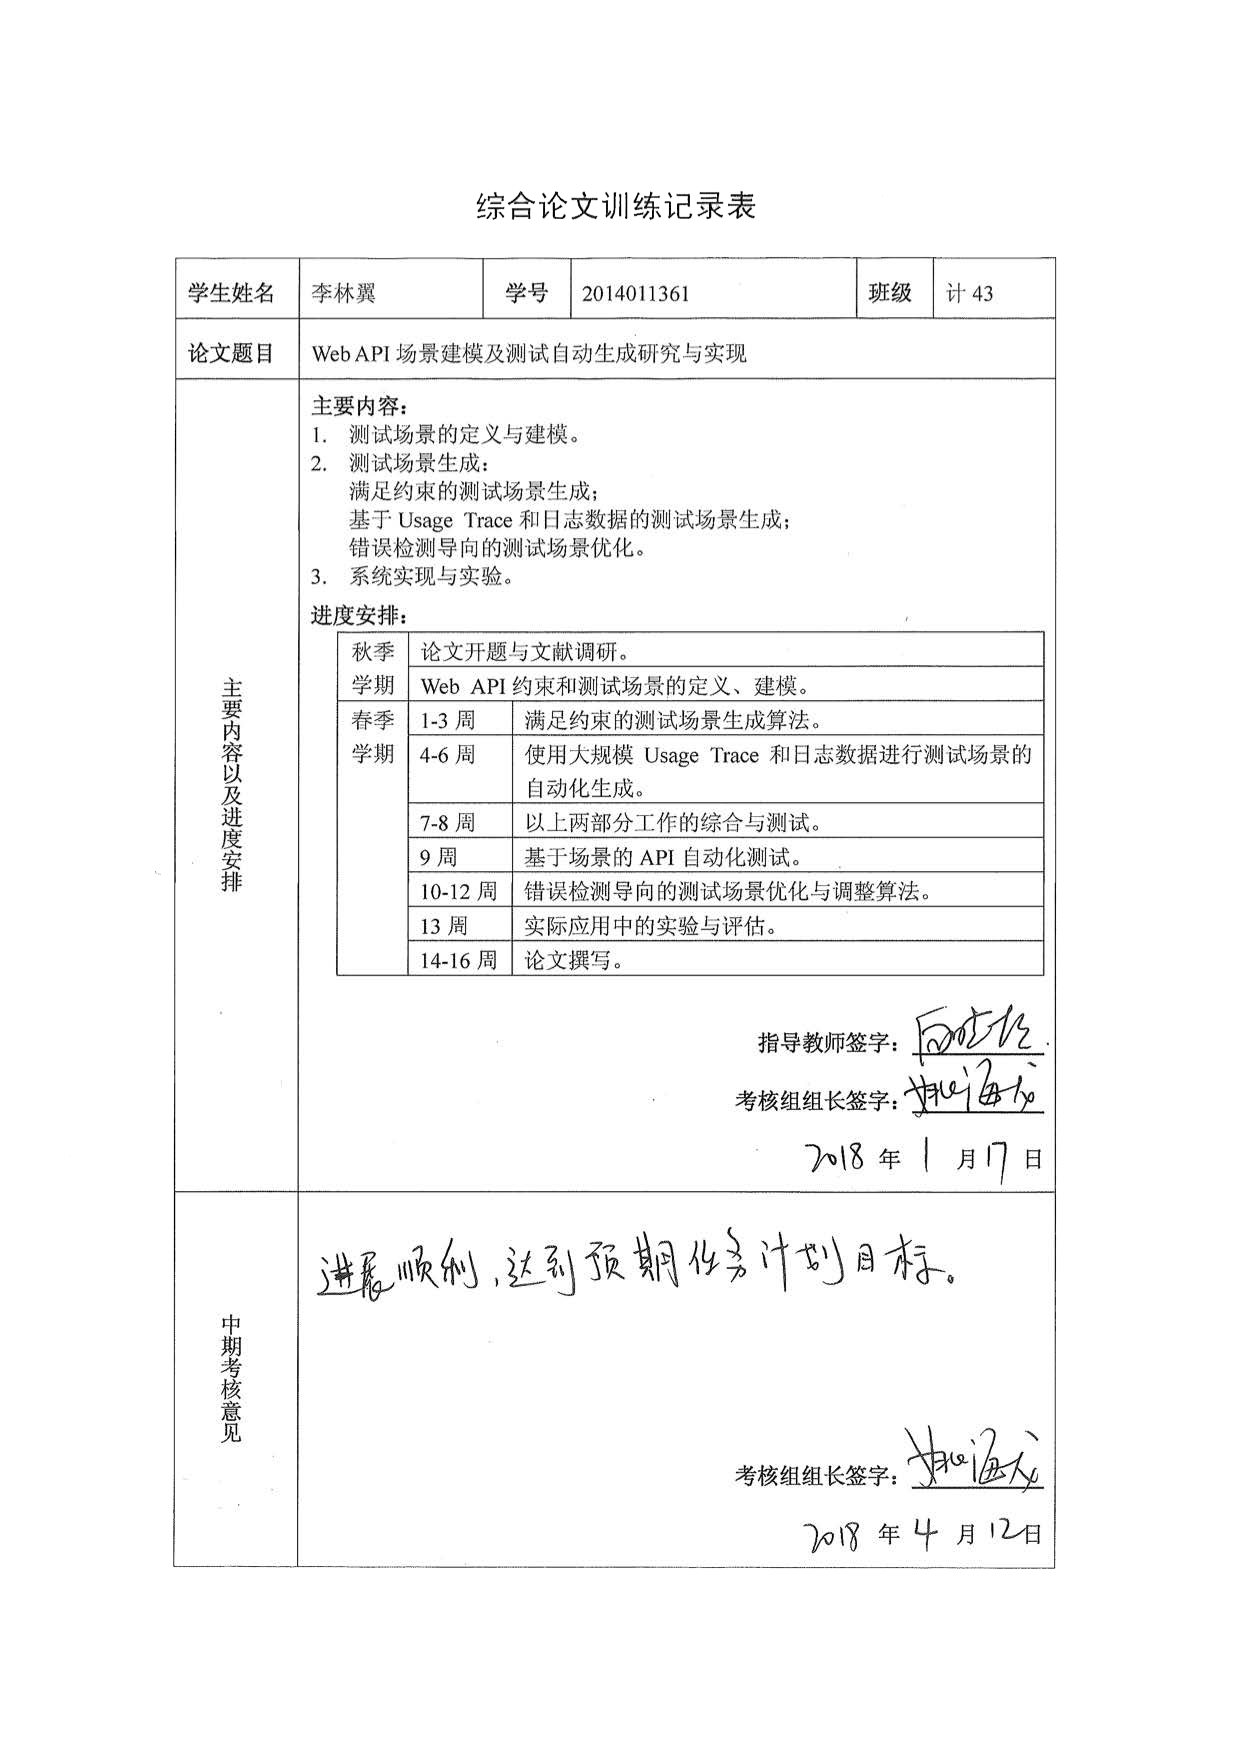
\includepdf[pages=-]{scan-record.pdf}
\end{document}
